\appendix


\chapter{User Walkthroughs}\label{app:user-walkthrough}

This section will go through each of the acceptance tests outlined in Section~\ref{sec:acc-tests} and provide the evidence that they pass. This evidence will be given in the form of:

\begin{itemize}
  \item Smart contract transaction logs from the Sepolia test-net. These are public at \small\url{https://sepolia.etherscan.io/address/0x2899dab55a4a20d698062bbf4d4ce9f1073ce052}\normalsize. The smart contract code was uploaded so all functions called and data uploaded are visible.
  \item Snippets of logs written that correspond to certain actions. For example, receiving a message over the network.
  \item Screenshots to show changes being reflected in the user interface.
\end{itemize}

\newparagraph
For this the game will be a simple folder of text files that we can easily compare to show correctness.

\small
\begin{itemize}
  \item \g{1} = [title="User WT", version="1.0", developer="tcs1g20",\newline uploader=0xfBC8D99Bb9ab8F781fF04F9b45Fe5c97AACE1916, previousVersion=None, price=0, rootHash=`']
  \item \g{2} = [title="User WT", version="2.0", developer="tcs1g20", previousVersion=\g{1}, price=0,\newline uploader=0xfBC8D99Bb9ab8F781fF04F9b45Fe5c97AACE1916, rootHash=`']
\end{itemize}
\normalsize


\chapter{Introduction}\label{sec:problem}

Millions of worldwide users enjoy video games, which are large pieces of software that require complex platforms to distribute them, which results in them being generally provided by multinational corporations. However this approach often results in these platforms:

\begin{itemize}
  \item taking a large cut of revenue from developers\footnote{Steam take a 30\% cut~\cite{marks_report_2019,brown_valve_2021}},
  \item being prone to censorship from entities like governments\footnote{See the Chinese version of Steam~\cite{noauthor_steam_nodate-1}},
  \item relying on a single platform to stay active, distribute games and maintain a user's ownership\footnote{The Nintendo eShop closing down prevents users from accessing games~\cite{noauthor_nintendo_2022}}.
\end{itemize}

\section{Objectives}

Modern web ideas revolve around taking power away from large corporations and having platforms that are built, run and maintained by those who use them.
This project aims to produce a proof-of-concept, distributed video game marketplace that will allow developers to continuously release and update their games on a public network such that they can be purchased and downloaded by other users.

\section{Scope}

This project will strictly focus on creating a distributed platform in which users can upload, purchase and share games and will consist of the following components:

\begin{enumerate}
  \item An Ethereum smart contract that will allow us to maintain a library of games that can be queried and added to by any user. This will then be deployed to an Ethereum test-net.
  \item A local application to be run by users to interact with the smart contract and allow them to join a peer-to-peer network where they can download and upload games.
\end{enumerate}

\newparagraph
This project will not present methods for preventing or stopping the distribution of illegal content or include tangentially related features such as achievements, or message boards.

\chapter{Background Research}

This chapter describes two distributed-web technologies that allows user to connect over large, decentralised networks and overcome issues of distributing data and building trust.


\section{BitTorrent}

BitTorrent~\cite{kaune_unraveling_2010,pouwelse_bittorrent_2005} is the most popular p2p file-sharing platform, in which users will barter for chunks of files by downloading and uploading them in a tit-for-tat fashion, such that peers with a high upload rate will typically also have a high download rate. For a user to download data from BitTorrent they would:

\subsection{Download Protocol}

\begin{enumerate}
  \item Find the corresponding \.torrent file that contains metadata about the torrent such as the location of a tracker, file information such as name, size and path in the directory.
  \item The user will find peers also interested in that torrent through a tracker and will establish connections with them.
  \item The data is split into constant-sized blocks and are downloaded individually. BitTorrent uses a tit-for-tat mechanism that incentivises users to contribute by providing preferable treatment to nodes who upload data as well.
  \item The user will download blocks based upon the following priority:
        \begin{enumerate}
          \item \textbf{Strict Priority} Data is split into pieces and sub-pieces with the aim that once a given sub-piece is requested then all of the other sub-pieces in the same piece are requested
          \item \textbf{Rarest First} Aims to download the piece that the fewest peers have to increase supply.
          \item \textbf{Random First Piece} When a peer has no pieces, it will try to get one as soon as possible to be able to contribute.
        \end{enumerate}
  \item The node will continuously upload blocks it has while active.
\end{enumerate}

\subsection{Availability}

It is commonly suggested that availability of torrents is the biggest issue surrounding BitTorrent as \textit{`38\% of torrents become unavailable in the first month'}~\cite{kaune_unraveling_2010} and that \textit{`the majority of users disconnect from the network within a few hours after the download has finished'}~\cite{pouwelse_bittorrent_2005}.
This paper~\cite{neglia_availability_2007} looks at how the use of multiple trackers for the same content and DHTs can be used to boost availability.



\section{Ethereum}

Ethereum is a Turing-complete, distributed, transaction-based blockchain that allows the deployment of decentralized applications through the use of smart contracts. Ether is the currency used on Ethereum and can be traded between accounts and is used to execute smart contract code on the network. 

\subsection*{Smart Contracts}

A smart contract is an executable piece of code, written in Solidity, that will automatically execute on every node in the Ethereum network when certain conditions are met. Smart contracts are enforced by the blockchain network and remove the need for intermediaries and reduce the potential of contractual disputes.
\x
Gas is used to measure the computational effort of running a smart contract and must be paid, in Ether, before being processed and added to the blockchain. This helps prevent DoS attacks and provides economic incentives for users to behave in a way that benefits the whole network.

\subsection*{Example Use Cases}

Some examples of applications that can be deployed to the Ethereum network are:

\begin{itemize}
  \item Financial applications, such as decentralised exchanges and payment systems,
  \item supply chain management and tracking,
  \item voting and governance systems,
  \item unique digital asset systems, and
  \item data storage and sharing platforms.
\end{itemize}

\chapter{Project Management}

\subsection*{Risk Assessment}

% \paragraph*{Difficult with blockchain development}

% Some of the difficulties I found with blockchain development were:

% \begin{itemize}
%   \item 
% \end{itemize}

\paragraph*{The application is not finished}
Section~\ref{tab:sprint-3} shows the scoped requirements that were not met and Section~\ref{sec:design-lim} shows some of the limitations within my design when compared to similar platforms. However, use of MoSCoW prioritisation and sprint planning meant I was still able to produce a largely functional application that met the majority of the requirements and having a cut off point for implementation ensured I had sufficient time to complete this report.
\x
One reason for not finishing was the size of the project, which took a considerable amount of time to implement and test. Table~\ref{tab:cloc} shows a breakdown of the source code.

\begin{longtable}{ r r r r }
  \toprule
  \textbf{Language} & \textbf{Files} & \textbf{Comments} & \textbf{Code}
  \\\midrule\midrule
  Go
  & 44
  & 683
  & 4621
  \\
  Go Tests
  & 29
  & 791
  & 3205
  \\
  Vue.js Components
  & 18
  & 147
  & 2855
  \\
  JavaScript
  & 19
  & 74
  & 209
  \\
  Solidity
  & 1
  & 30
  & 51
  \\\bottomrule\bottomrule
  \caption{The lines of code written for this project calculated using CLOC~\cite{noauthor_aldanialcloc_nodate} excluding any auto-generated code.}
  \label{tab:cloc}
\end{longtable}

\paragraph*{Lack of large-scale testing infrastructure}
Testing distributed applications is challenging due to many factors, such as having to source homogenous devices, having access to networks that would allow me host a peer, and more. However, several useful results were produced from the benchmarks (Section~\ref{sec:benchmark}) and acceptance tests (Section~\ref{sec:acc-tests}) that can be used to improve the application. If this project were to move forward then testing it on a large-scale would be essential.
\section{Sprint Plans}

\newcommand{\yes}{\cellcolor{green!30}YES}
\newcommand{\started}{\cellcolor{yellow!50}STARTED}
\newcommand{\no}{\cellcolor{red!30}NO}

The use of sprints was essential in managing my time and ensuring that I was working on the most important aspects of my project first. The use of MoSCoW priortisation and by then dividing my requirements into logical groups I was able to effectively target key aspects of my application in bulk. The use of test-driven development~\cite{beck_test-driven_2003} meant that at the end of each sprint, each piece of code I wrote was tested and I could move on.
\x
For each sprint we will detail the planned requirements, whether they were completed or not, as well as any general comments about that sprint.

\subsection{Sprint 1}

I anticipated that the P2P game distribution network would be the most complex and time consuming set of requirements in this project so I decided to focus on it for this first sprint. Table~\ref{tab:sprint-1} shows the requirements included for Sprint 1 and whether they were completed or not.
\x
This sprint was largely problem-free as I didn't have much to learn to be able to complete this and could rely heavily on my design to structure my implementation.

\begin{longtable}{p{0.12\textwidth} p{.13\textwidth} p{.6\textwidth}}
  \toprule
  \textbf{Req.} & \textbf{Complete} & \textbf{Evidence/Reasoning}
  \\\midrule\midrule
  \reqref{F-M7}
  & \yes
  & Unit tests for the model/net/tcp package and the peer count benchmark tests.
  \\
  \reqref{F-M8}
  & \yes
  & Unit tests for the model/net/peer/message\_handlers file test the handling of structured messages and the structured responses sent back. 
  \\
  \reqref{F-M9}
  & \yes
  & All benchmark tests show the downloading of data to a large scale.
  \\
  \reqref{F-M10}
  & \yes
  & Unit tests to show incorrect messages being rejected.
  \\
  \reqref{F-M11}
  & \yes
  & User walkthrough shows the download of a game in its entirety. 
  \\
  \reqref{F-M12}
  & \started
  & The algorithm to generate a hash tree and the using of it to download data was implemented but no way to upload it anywhere.
  \\\midrule\midrule
  \reqref{NF-M2}
  & \yes
  & User walkthrough ... shows that any user can establish a connection with any other user.
  \\
  \reqref{NF-S1}
  & \started
  & Users will form many connections concurrently and optimisations were made using the producer/consumer pattern to complete actions like inserting data, or reqeusting data.
  \\\bottomrule\bottomrule
  \caption{Requirements included for Sprint 1}
  \label{tab:sprint-1}
\end{longtable}

\subsection{Sprint 2}

Sprint 2 was about increasing the scope of the application by focusing on two main aspects:

\begin{enumerate}
  \item The integration with Ethereum using a Smart Contract, and
  \item Allowing users to interface with the application via a GUI.
\end{enumerate}

\vspace{2mm}\noindent
This sprint had a much slower start compared to the first one as I was largely unfamiliar with smart contract development and the related packages needed to interface with them. On top of this, I considered several UI framework's before settling on my final choice which increased the length of this sprint.
\x
Table~\ref{tab:sprint-2} shows the requirements pitched for Sprint 2 and whether or not they were completed.

\begin{longtable}{p{0.12\textwidth} p{.13\textwidth} p{.6\textwidth}}
  \toprule
  \textbf{Req.} & \textbf{Complete} & \textbf{Evidence/Reasoning}
  \\\midrule\midrule
  \reqref{F-M1}
  & \yes
  & Unit tests for the Library smart contract and user walkthrough ... show the ability to upload game metadata to Ethereum.
  \\
  \reqref{F-M2}
  & \yes
  & Unit tests for the Library smart contract and user walkthrough ... show the ability to upload an update to an existing game to Ethereum.
  \\
  \reqref{F-M3}
  & \yes
  & Unit tests for the Library smart contract show users of an existing game being given ownership of an updated version.
  \\
  \reqref{F-M4}
  & \yes
  & The smart contract was successfully deployed the Sepolia test-net~\cite{etherscanio_deployed_nodate}. All user walkthroughs will form connections to this smart contract.\\
  \reqref{F-M5}
  & \yes
  & Unit tests for the Library smart contract and user walkthrough ... show the successful purchase of a game.
  \\
  \reqref{F-M6}
  & \yes
  & Unit tests for the Library smart contract show a user being added to a mapping containing all users who have purchased the game.
  \\
  \reqref{F-M12}
  & \yes
  & Hash trees are now uploaded to IPFS and the CID is stored on Ethereum. 
  \\
  \reqref{F-S2}
  & \started
  & Basic pages were added according to Section~\ref{subsubsec:frontend}. These pages had little styling or reactivity but could perform the required basic functions. See Appendix~\ref{app:screenshots} for screenshots of the final versions.
  \\\midrule\midrule
  \reqref{NF-M1}
  & \yes
  & The use of the Ethereum blockchain means that no single user can control what is uploaded to the network.
  \\
  \reqref{NF-M3}
  & \yes
  & Developers can be uniquely identified using their Ethereum address. This should be made publically verifiable by the developers.
  \\
  \reqref{NF-M4}
  & \yes
  & Data stored on Ethereum is inherently immutable.
  \\
  \reqref{NF-M5}
  & \yes
  & Unit tests for the smart contract show the restriction that only the original uploader can release an update.
  \\\bottomrule\bottomrule
  \caption{Requirements included for Sprint 2}
  \label{tab:sprint-2}
\end{longtable}

\subsection{Sprint 3}

\begin{longtable}{p{0.12\textwidth} p{.13\textwidth} p{.6\textwidth}}
  \toprule
  \textbf{Req.} & \textbf{Complete} & \textbf{Evidence/Reasoning}
  \\\midrule\midrule
  \reqref{F-S1}
  & \yes
  & Users will validate each other's Ethereum address after forming a connection and unit tests for the model/net/peer/message\_handlers file show this being performed.
  \\
  \reqref{F-S2}
  & \yes
  & The UI was overall improved to improve the user experience.
  \\
  \reqref{F-S3}
  & \no
  & Users will track the blocks sent to them by each of their peers but this application has no mechanism for redeeming these. Due to time constraints, I was unable to implement a sufficient solution. Moreover, I felt that a micro-payment system, like present in Swam~\cite{hartman_swarm_1999}, would be a much better implementation.
  \\
  \reqref{F-S4}
  & \yes
  & Users will exchange the REQ\_PEERS/PEER commands to discover neighbouring peers.\newline
  However a better implementation might have the developer of the game be able to provide a list of peers who have the game. This would allow a user to easily find peers who are interested in the same content.
  \\
  \reqref{F-C1}
  & \no
  & Due to time constraints I was unable to implement this at all.
  \\
  \reqref{F-C2}
  & \yes
  & Game assets are uploaded to IPFS and the CID is stored with the game metadata on Ethereum.
  \\\midrule\midrule
  \reqref{NF-S1}
  & \yes
  & Benchmark tests show the scalability of my application by varying certain parameters and that the target file size can be downloaded within an acceptable best-case.
  \\
  \reqref{NF-S2}
  & \yes
  & Changes to the UI made it more interactive and easier to navigate. Designs were inspired by pages from existing platforms to make the UI feel familiar. See Appendix~\ref{app:screenshots} for screenshots of the final versions.
  \\
  \reqref{NF-C1}
  & \no
  & Completing this requirement would be incredibly complex and was decided against being completed. Preventing the distribution of illegal content is an important consideration moving forward to help keep the platform safe.
  \\
  \reqref{NF-C2}
  & \yes
  & A help page was included answering some questions that new users may have about the application.
  \\\bottomrule\bottomrule
  \caption{Requirements included for Sprint 3}
  \label{tab:sprint-3}
\end{longtable}


\section{Gantt Chart}

A Gantt chart was used to give myself a high-level overview of how my time should be spent so that I would have appropriate time to complete the necessary aspects of this project. This was useful in prioritising different aspects and knowing when to plan deadlines for myself (for example, having a hard cut-off point for my implementation).
\x
Figure~\ref{fig:gantt-chart-1} shows the Gantt chart for this project up util the progress report submission, which includes the planning and design phases.

\begin{figure}[H]
  \centering
  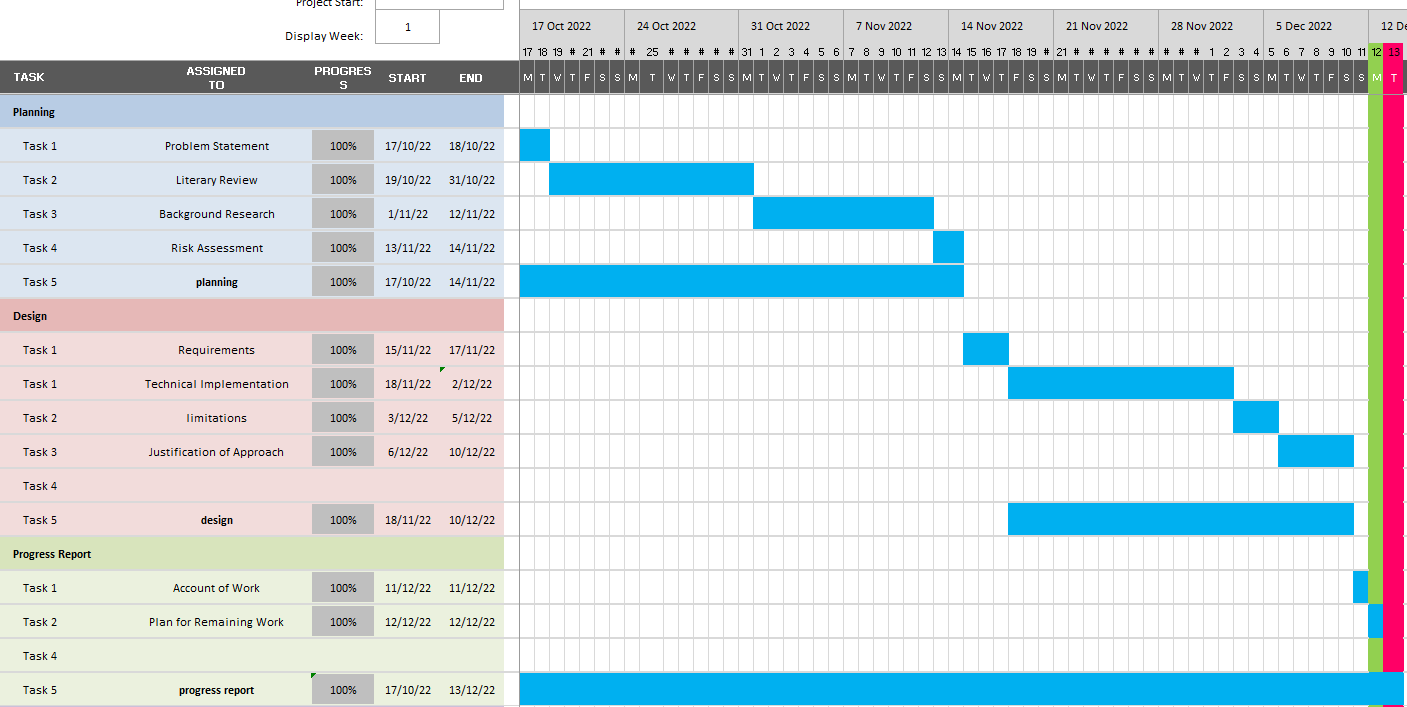
\includegraphics[width=\textwidth]{assets/images/charts/gantt/progress.png}
  \caption{Gantt Chart leading up to the progress report}
  \label{fig:gantt-chart-1}
\end{figure}

\noindent Figure~\ref{fig:gantt-chart-2} shows the Gantt chart for the implementation phase of this project. The implementation phase was split into three sprints, as detailed in Section~\ref{sec:sprints}, each with their own planning phase.

\begin{figure}[H]
  \centering
  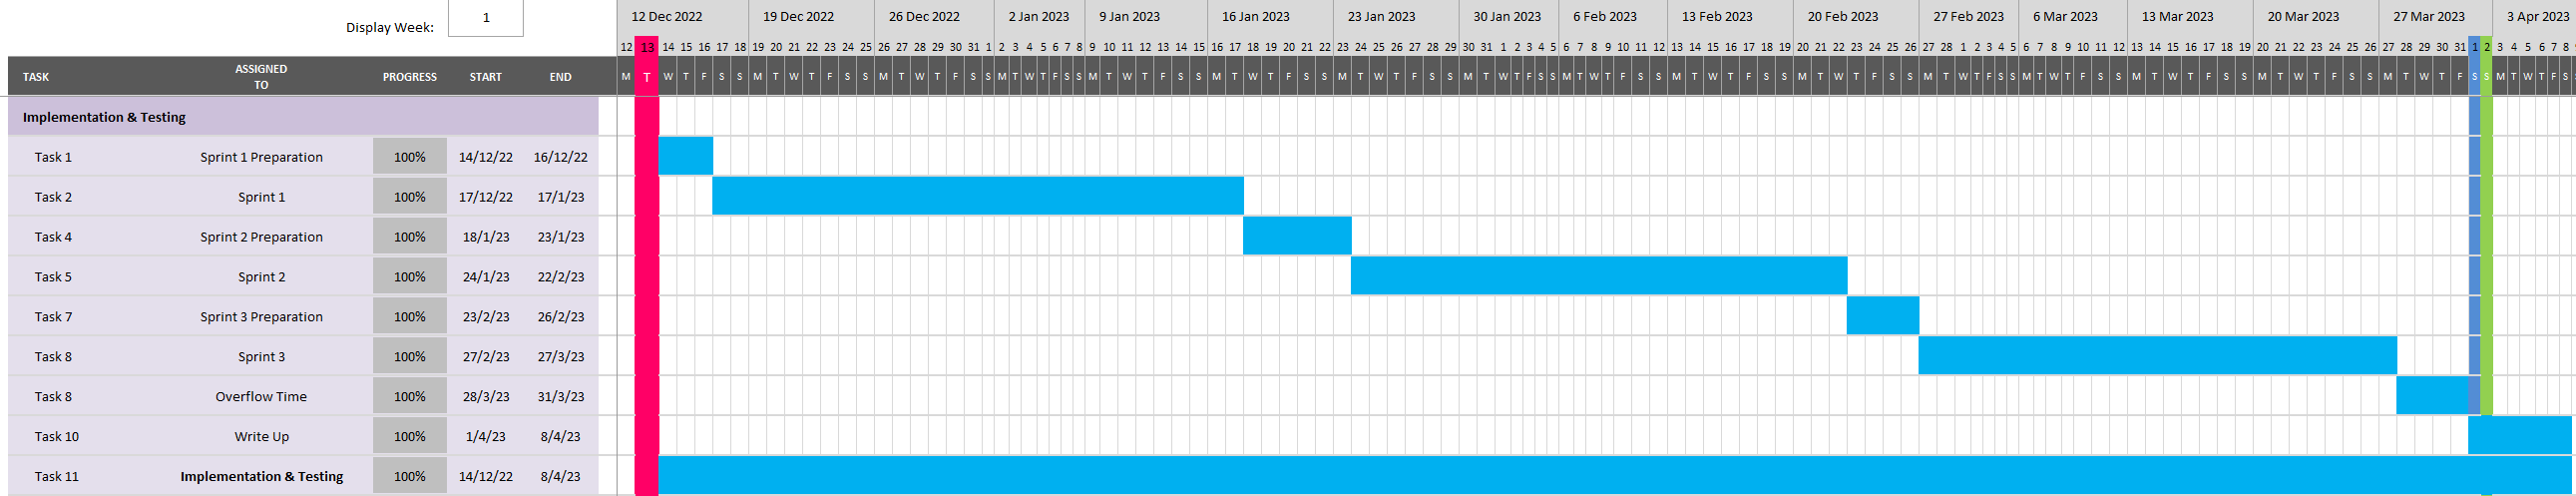
\includegraphics[width=\textwidth]{assets/images/charts/gantt/impl.png}
  \caption{Gantt Chart showing the three sprints}
  \label{fig:gantt-chart-2}
\end{figure}

\noindent Figure~\ref{fig:gantt-chart-3} shows the Gantt chart for the final testing and evaluation phases of my application. As I used test-driven development, the testing phase only needed to consist of acceptance and benchmark testing among some other fixes. 

\begin{figure}[H]
  \centering
  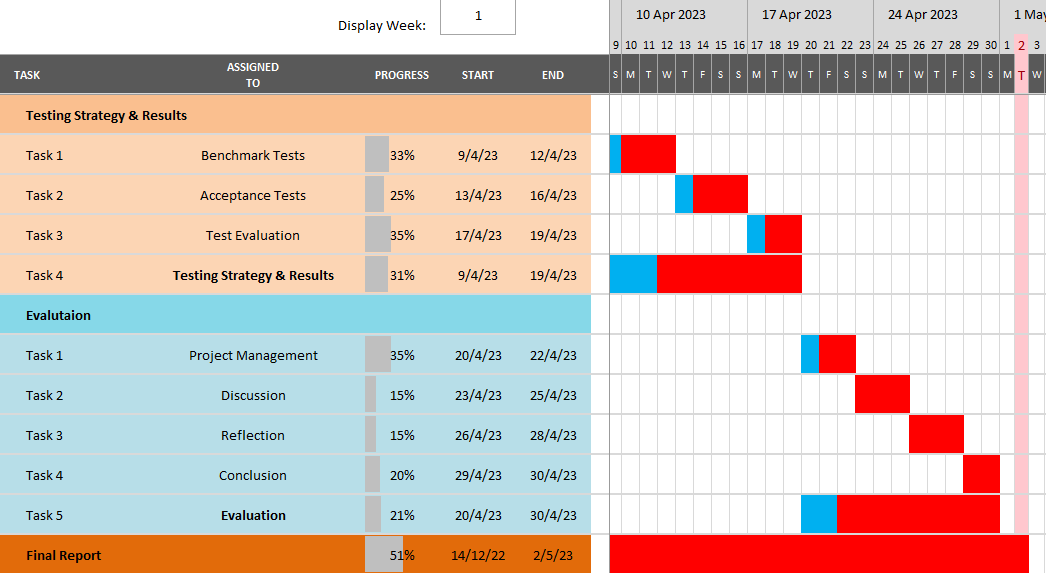
\includegraphics[width=\textwidth]{assets/images/charts/gantt/testing-eval.png}
  \caption{Gantt Chart showing the final testing and evaluation}
  \label{fig:gantt-chart-3}
\end{figure}
% \section{Work to Date}

My work has primarily been on research, looking at how blockchain has been used to build and supplement cloud storage systems as well as how various peer-to-peer functioned and performed. 
I have proposed a design for the application to be built on the EVM. 

\begin{figure}[ht]
  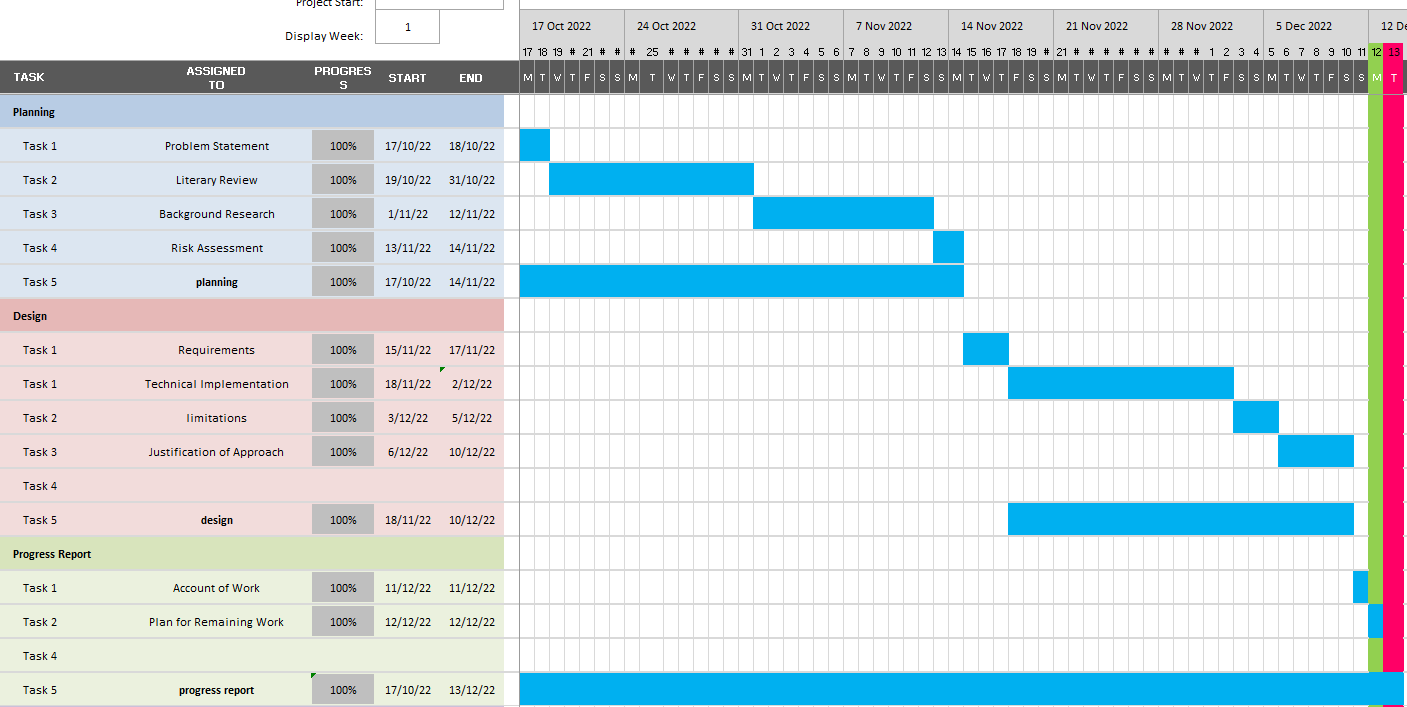
\includegraphics[width=\textwidth]{assets/images/charts/gantt/progress.png}
  \caption{A Gantt chart for my work up until the progress report.}
\end{figure}

% \section{Plan of Future Work}

Below is a high level plan of the work I have remaining. At the end of each section, I will write up the initial draft of that section in my final report based upon notes made throughout the project.

\subsection*{Implementation \& Testing}
This phase I will use the agile development methodology to build my application. My sprints will all be structured into three phases:
\vspace{1mm}

\begin{enumerate}
  \item \textbf{Preparation} Deciding on the set of requirements to complete and making any initial design decisions and diagrams,
  \item \textbf{Implementation} using test-driven development, I will work on requirements based on their prioritization, and
  \item \textbf{Review} I will discuss the completed work in that sprint including design choices, what was completed, and any issues.  
\end{enumerate}

\vspace{1mm}\noindent By using a preparation and review phase with each sprint, I can make detailed notes on my implementation as I go so when I come to write the full report I have a strong starting point.

\begin{figure}[ht]
  \centering
  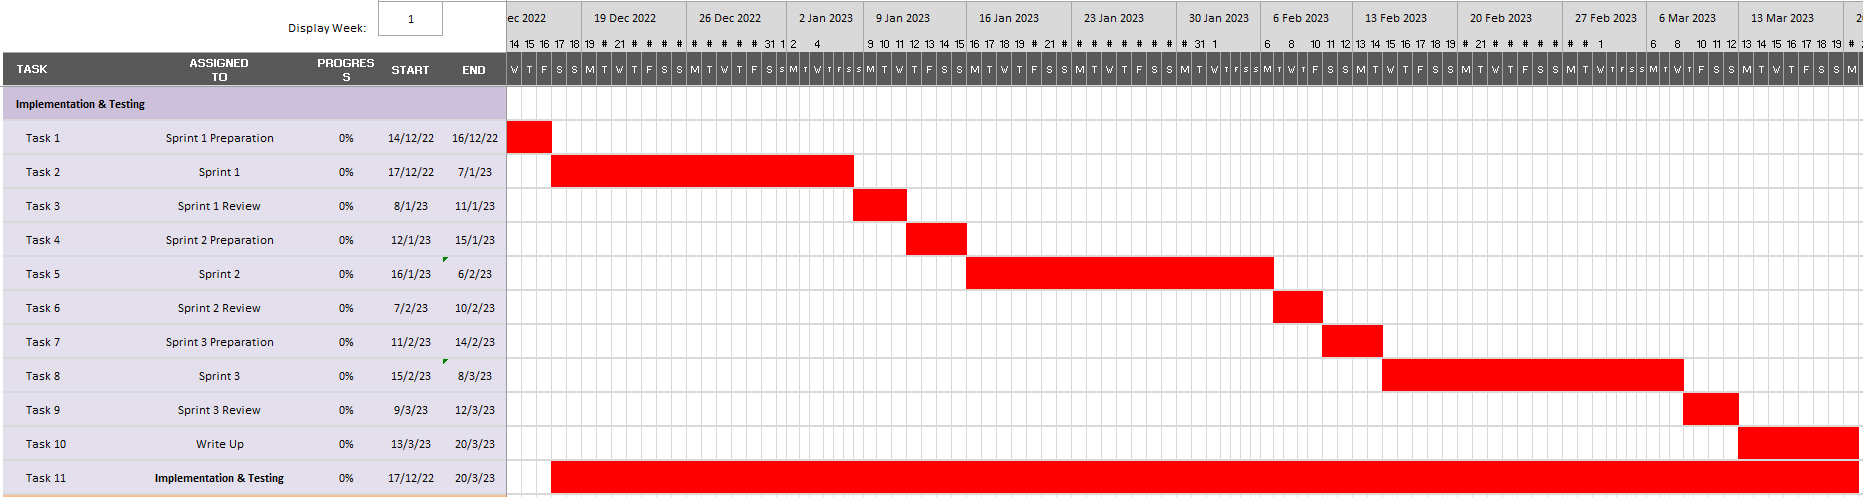
\includegraphics[width=\textwidth]{assets/images/charts/gantt/implementation-testing.png}
  \caption{The plan for my three sprints}
\end{figure}

\subsection*{Testing Strategy and Results}
This phase will consists of several sections:

\begin{enumerate}
  \item \textbf{Testing Strategy} The approach I used for writing tests throughout the implementation phase and how these were used to evaluate the completion of the requirements set out in Section~\ref{subsec:requirements}. 
  \item \textbf{Test Results} A report on the results of my automated and manual testing.
\end{enumerate}

\subsection*{Evaluation}
This phase will have me evaluating how successful my project was, as a whole, by focusing on several key areas:

\begin{enumerate}
  \item \textbf{Project Organisation} How successfully did I structure my time in this project?
  \item \textbf{Outcome of the Application} How successful was my application in regards to a solution to the problem set out in Section~\ref{sec:problem} and in terms of the requirements set out in Section~\ref{subsec:requirements}?
  \item \textbf{Limitations and Future Improvements} What were the limitations of my project and what would I change about it if I had more time or were to start again?
\end{enumerate}

\begin{figure}[ht]
  \centering
  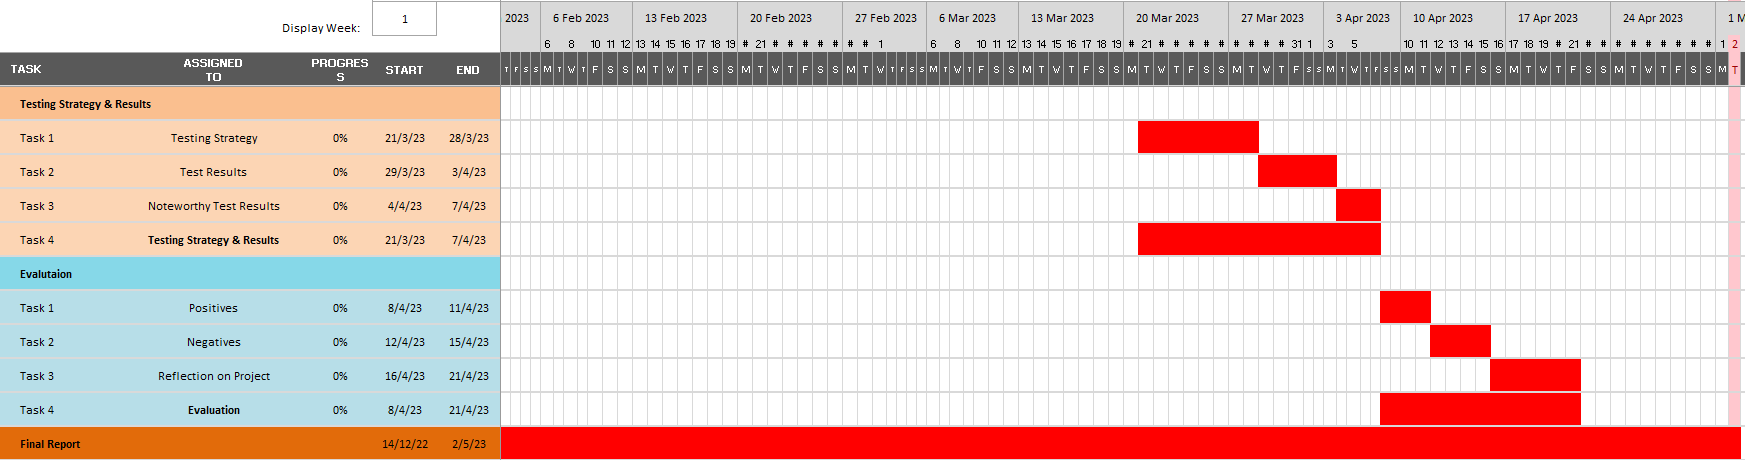
\includegraphics[width=\textwidth]{assets/images/charts/gantt/testing-evaluation.png}
  \caption{The plan for my testing and evaluation phases}
  \label{fig:final-gantt}
\end{figure}

\subsection*{Leftover Time}

At the end of my project, I've left some time unallocated to account for certain tasks that may take longer as well as the writing up of my final report. This should leave me with an acceptable amount of time to finish the project despite some setbacks.


\chapter{Literature Review}\label{ch:lit-review}

This section will be used to examine the literature surrounding the distributed storage of data. Initially I will look at various distributed file-sharing protocols and then how blockchain has been used to enhance them.


\section{P2P File Sharing}

These applications involve a distributed network of computers that share data with each other without the need for a central party. Table~\ref{tab:lit-review-p2p} shows some example p2p file-sharing networks.
\x
One of the main issues with these networks come from their anonymity property in that you can never fully trust that what you're downloading isn't malicious. On top of this, these platforms don't offer a way for user to pay for the content they are downloading, which means that legal, proprietary content is rarely distributed over them.

\begin{longtable}{ p{0.15\textwidth} p{0.8\textwidth} }
  \toprule
  \textbf{System} & \textbf{Description of Solution}
  \\\midrule\midrule
  IPFS~\cite{benet_ipfs_2014}
  & IPFS is a content-addressable, block storage system which forms a Merkle DAG, a data structure that allows the construction of versioned file systems, blockchains and a Permanent Web.
  %
  \x
  BitTorrent~\cite{pouwelse_bittorrent_2005}
  & BitTorrent is a p2p file-sharing system that has user bartering for chunks of data in a tit-for-tat fashion, which provides incentive for users to contribute to the network. More on BitTorrent can be found in Section~\ref{sec:bittorrent}
  %
  \x
  AFS~\cite{morris_andrew_1986,howard_scale_1988}
  & The Andrew File System was a prototype distributed system by IBM and Carnegie-Mellon University in the 1980s that allowed users to access their files from any computer in the network.
  %
  \x
  Napster~\cite{saroiu_measurement_2001}
  & Napster uses a cluster of centralized servers to maintain an index of every file currently available and which peers have access to it. A node will maintain a connection to this central server and will query it to find files; the server responds with a list of peers and their bandwidth and the node will form a connection with one or many of them and download the data.
  %
  \x
  Gnutella~\cite{saroiu_measurement_2001}
  & Gnutella nodes form an overlay network by sending \textit{ping-pong} messages. When a node sends a \textit{ping} message to their peers, each of them replies with a \textit{pong} message and the \textit{ping} is forwarded to their peers. To download a file, a node will flood a message to its neighbors, who will check if they have and return a message saying so; regardless, the node will continue to flood their request till they find a suitable node to download off of.
  \\\bottomrule
  \caption{\textit{Various global distributed file systems.}}
  \label{tab:lit-review-p2p}
\end{longtable}

\section{Blockchain-Based Cloud Storage}

In table~\ref{tab:blockhain cloud storage}, I detail some examples of how blockchain has been used to solve problems within cloud storage systems. One interesting finding from these papers~\cite{sukhodolskiy_blockchain-based_2018,hasan_cloud_2019} is that blockchain can been used to provide additional services to cloud storage systems, such as monitoring access control or helping to verify the integrity of the data on these systems.

\begin{longtable}{ p{0.35\textwidth} p{0.6\textwidth} }
  \toprule
  \textbf{Paper} & \textbf{Description of Solution}
  \\\midrule\midrule
  Blockchain Based Data Integrity Verification in P2P Cloud Storage~\cite{yue_blockchain_2018}
  & This paper uses Merkle trees to help verify the integrity of data within a P2P blockchain cloud storage network as well as looking at how different structures of Merkle trees effect the performance of the system.
  %
  \x
  Deduplication with Blockchain for Secure Cloud Storage~\cite{li_deduplication_2018}
  & This paper describes a deduplication scheme that uses the blockchain to record storage information and distribute files to multiple servers. This is implemented as a set of smart contracts.
  %
  \x
  Block-secure: Blockchain based scheme for secure P2P cloud storage~\cite{li_block-secure_2018}
  & A distributed cloud system in which users divide their own data into encrypted chunks and upload those chunks randomly into the blockchain, P2P network. 
  %
  \x
  Blockchain-Based Medical Records Secure Storage and Medical Service Framework~\cite{chen_blockchain-based_2018}
  & Describes a secure and immutable storage scheme to manage personal medical records as well as a service framework to allow for the sharing of these records.
  %
  \x
  A Blockchain-Based Access Control System for Cloud Storage~\cite{sukhodolskiy_blockchain-based_2018}
  & This paper describes a method for using blockchain to facilitate the access control over a cloud storage system. The blockchain stores an immutable record of all `\textit{meaningful security events}', such as key generation, access policy, assignment, etc.
  %
  \x
  Cloud Data Provenance using IPFS and Blockchain Technology~\cite{hasan_cloud_2019}
  & Uses blockchain technology and IPFS to provide an efficient way to securely store provenance~\footnote{Provenance data are access logs of stored data that can trace the integrity of data and will contain private user information.} data such that it is out of reach of adversaries, but can be used to verify the integrity of data on a cloud storage system. 
  \\\bottomrule\bottomrule
  \caption{\textit{Examples of blockchain cloud storage systems~\cite{sharma_blockchain_2021} }}
  \label{tab:blockhain cloud storage}
\end{longtable}



\section{Overview}
\chapter{Design}


\input{sections/5-design/analysis/stakeholders.tex}
\input{sections/5-design/analysis/requirements.tex}

\section{Design Considerations}

This section will give a high-level design showing how each of the functional requirements can be met by considering key functions for the applications.

\input{sections/5-design/considerations/data.tex}
\input{sections/5-design/considerations/eth.tex}
\input{sections/5-design/considerations/p2p.tex}

\section{Architecture}

This application uses the Model-View-Controller MVC pattern to structure the application to create a separation of concern between the main layers of the application. Figure~\ref{fig:impl-layers} shows a high level overview of the architecture and below I discuss the purpose for each.

\begin{figure}[ht]
  \centering
  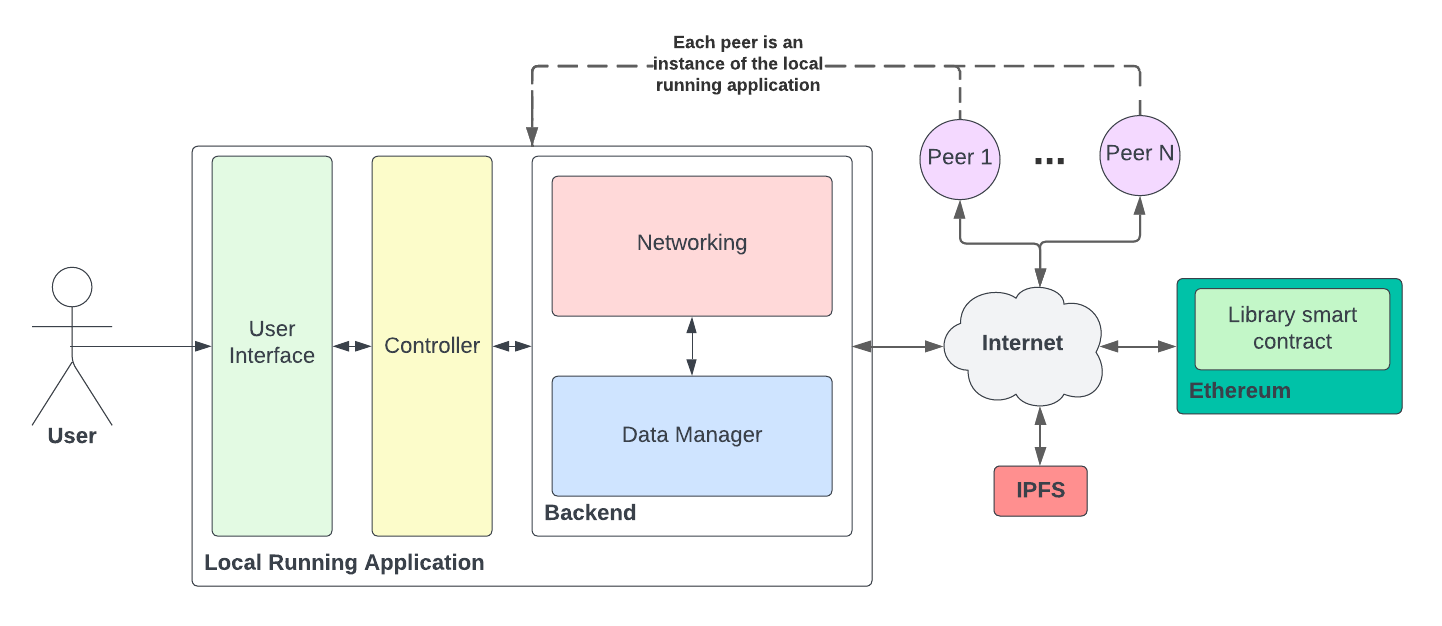
\includegraphics[width=.8\textwidth]{assets/images/diagrams/layers.png}
  \caption{The layers of the application}
  \label{fig:impl-layers}
\end{figure}

% layer entries

\input{sections/5-design/components/persistence/persistence.tex}
\input{sections/5-design/components/backend/backend.tex}
\input{sections/5-design/components/ui/frontend.tex}

\newpage

\section{Downloading a Game}

Figure~\ref{fig:p2p-interactions} shows the standard sequence of events used for a user to download a game from this application. The developer will upload a game that is purchased by a user; this user will then proceed to download the game off of the developer using the commands described in Section~\ref{subsubsec:commands}.
\x
Some important notes about this interaction are:

\begin{itemize}
  \item Identity verification happens immediately after forming a connection.
  \item Deferred requests are attempted when connecting to a new peer and after a timeout.
  \item Game ownership is checked upon the first BLOCK request.
\end{itemize}

\begin{figure}[!ht]
  \centering
  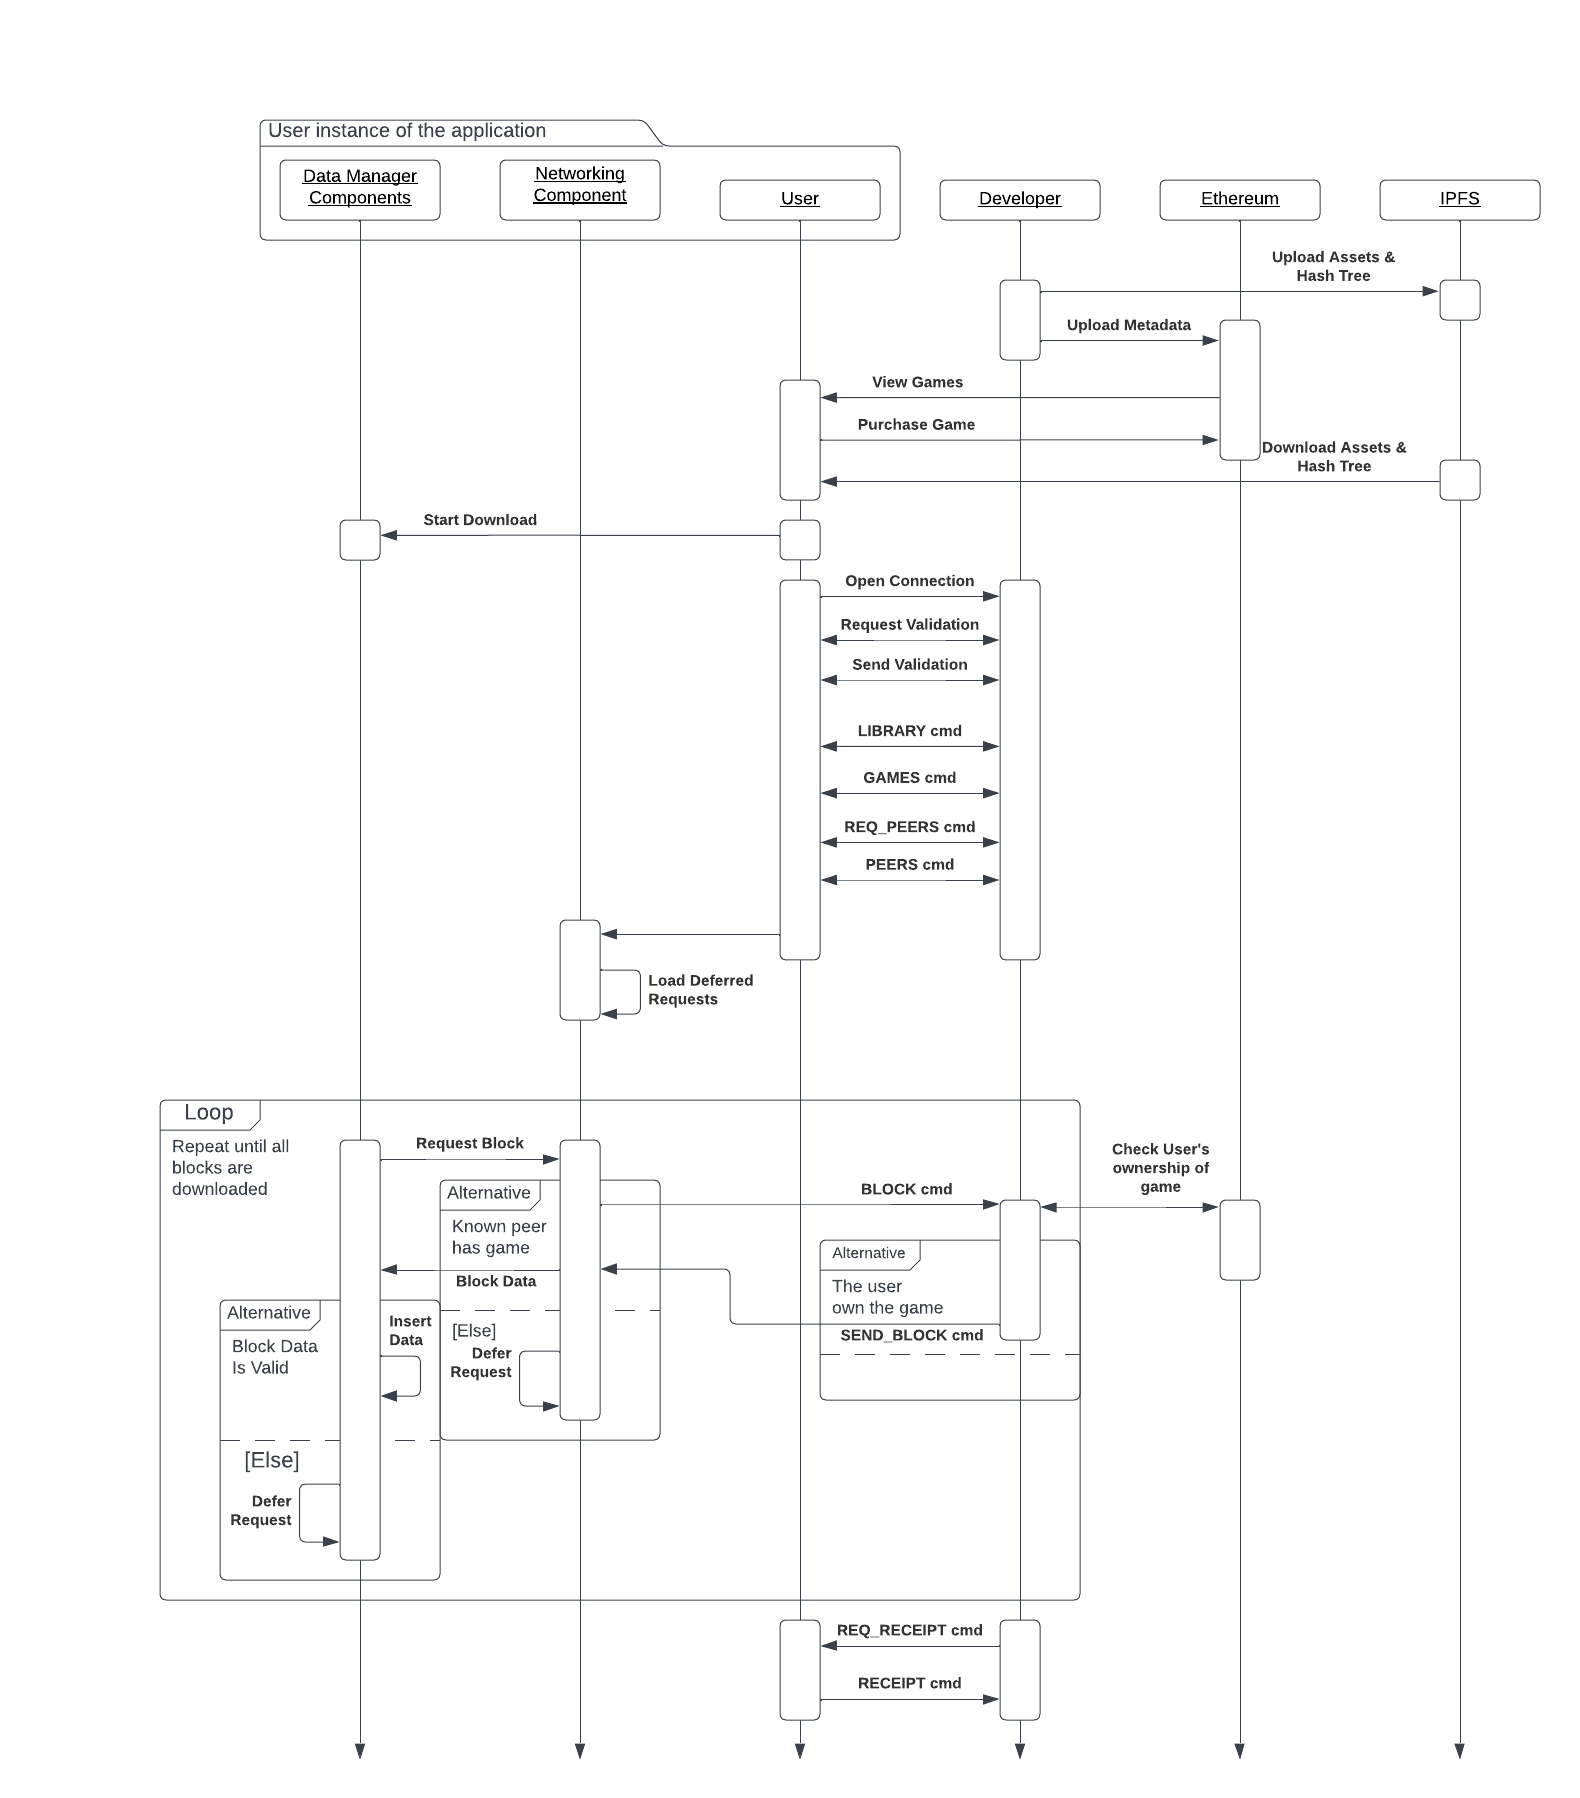
\includegraphics[width=\textwidth]{assets/images/diagrams/p2p-sequence.png}
  \caption{A sequence diagram showing the main interactions needed to download a game}
  \label{fig:p2p-interactions}
\end{figure}



\section{Benefits}\label{des:benefits}

This application presents the following benefits when compared with centralised game marketplaces:

\begin{itemize}
  \item \textbf{Privacy} A user's personal information and usage isn't collected. Traditional platforms require users to enter personal information and will actively collect data about a user's actions through the platform.
  \item \textbf{Ownership} A user's ownership of a game isn't tied to a single platform and use of Ethereum means that a user's ownership is upheld by all computers in the network.
  \item \textbf{Censorship} Similar to the previous point, no one party has control over the platform so it is much harder for third parties, such as governments, to restrict the content uploaded to it.
  \item \textbf{Profits} Developers and gamers communicate directly and this means developer's won't have to pay a hefty fee for a middle-man. This will result in potentially larger profits for the developers.  
\end{itemize}

\section{Limitations}\label{sec:design-lim}

This application presents the following limitations when compared with a centralised game marketplace:

\begin{itemize}
  \item \textbf{No Social Features} Social features, such as friends or achievements, were not included within the scope of this project.
  \item \textbf{Availability} Section~\ref{subsec:availability} highlights the issue of availability within P2P file-sharing systems and it is likely this platform will face similar issues.
  The use of a contribution system was implemented to help identify those users who have been contributing but there is no automatic rewards system\footnote{An example would be how the micro-payment system works in Swarm~\cite{hartman_swarm_1999}}.
  \item \textbf{Inefficient Updates} As updates are treated as individual games, they will require users to download the entire game again. This is highly inefficient and results in lots of duplicate data being downloaded.
  \item \textbf{Illegal Content} Currently there is no policy, automated or otherwise, to stop the distribution of illegal content. This is an incredibly complex problem to tackle and any obvious solution would risk violating the anti-censorship goal of this project. 
\end{itemize}
\chapter{Screenshots}\label{app:screenshots}

\begin{figure}[H]
  \centering
  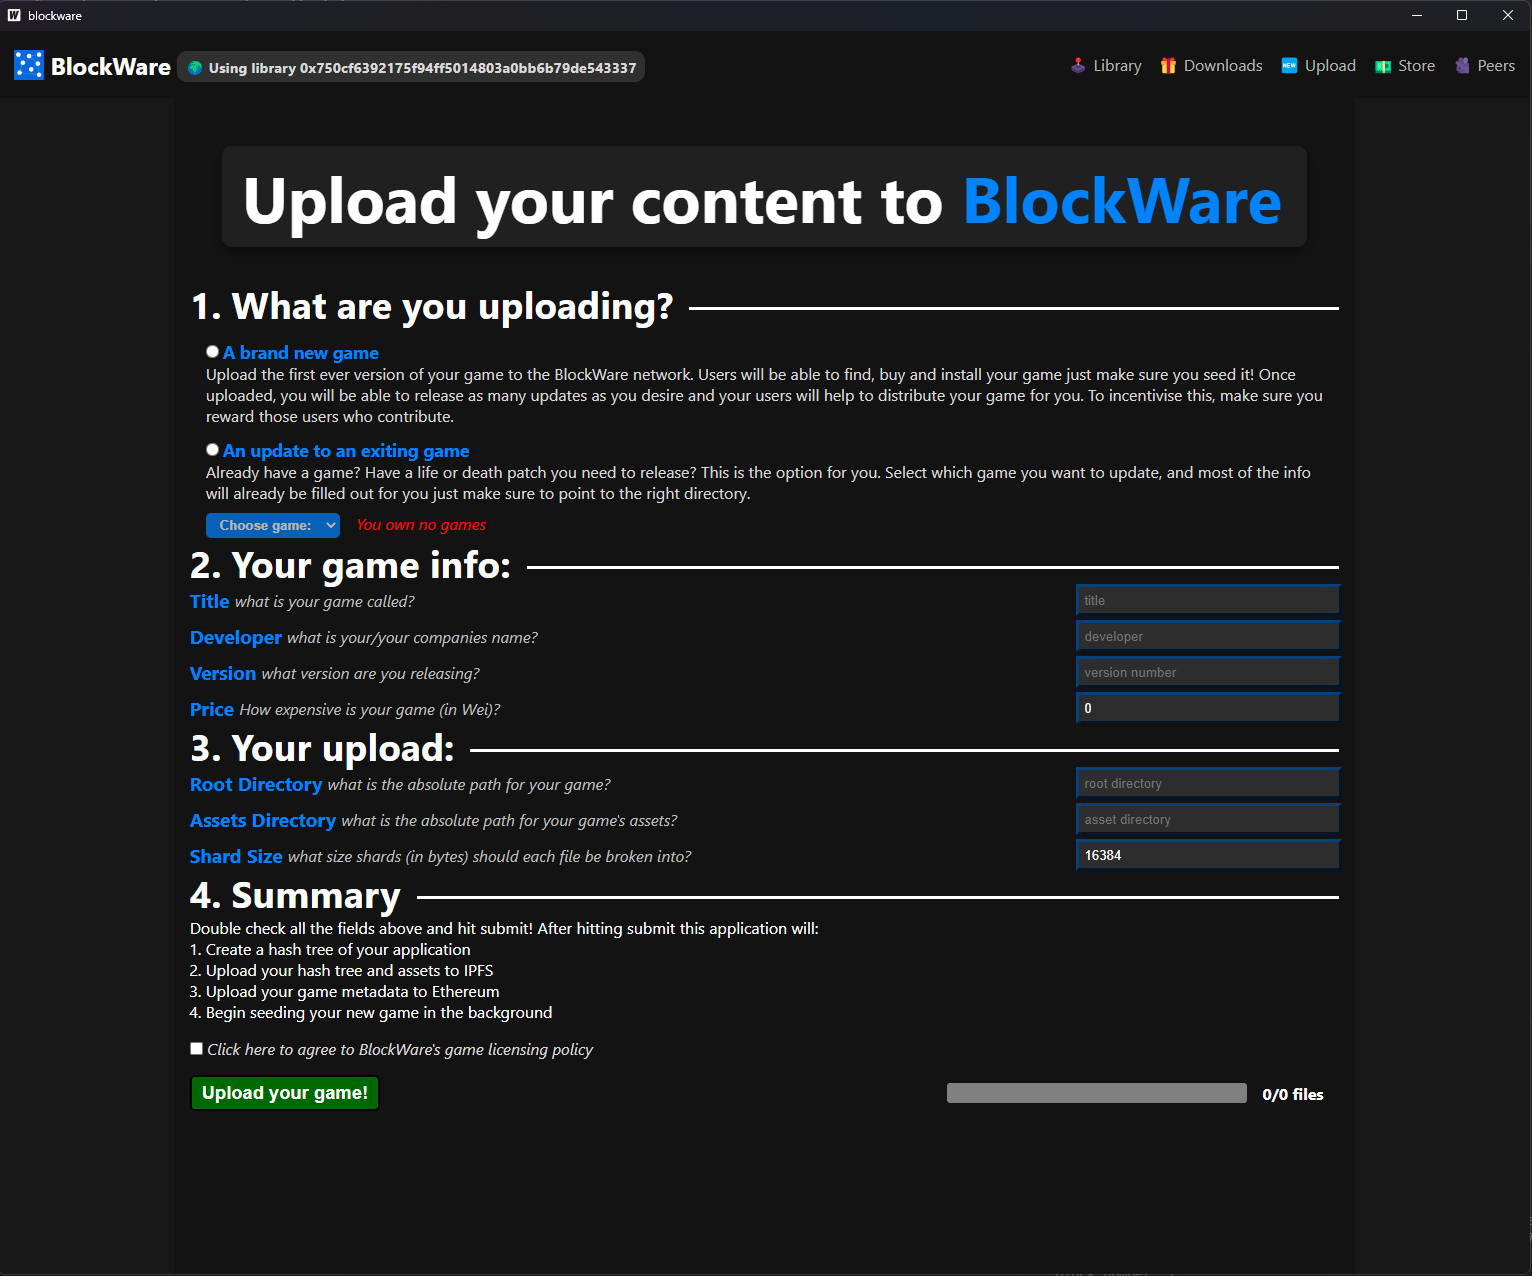
\includegraphics[width=0.9\textwidth]{assets/images/screenshots/upload.png}
  \caption{The page where users input the details about their game and can upload it to the Ethereum network. If a user wants to update a game they can choose from their uploaded games.}
\end{figure}

\begin{figure}[H]
  \centering
  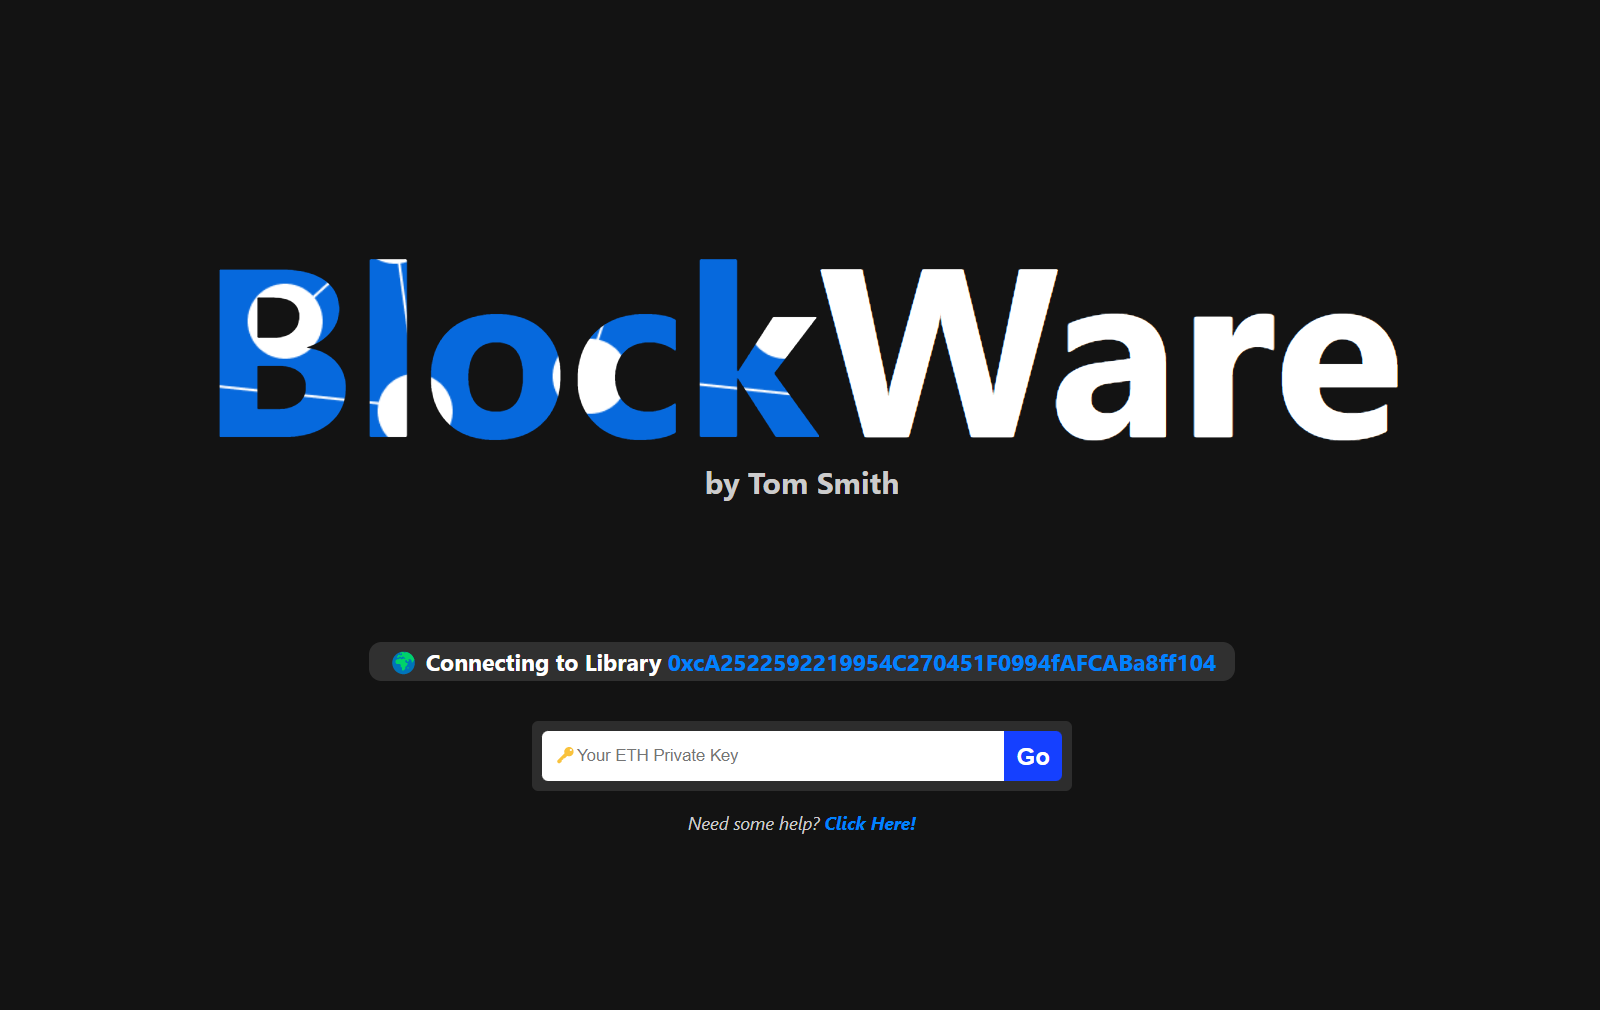
\includegraphics[width=0.9\textwidth]{assets/images/screenshots/login.png}
  \caption{The login page where a user will enter their Ethereum private key and connect to the BlockWare contract instance deployed to Sepolia. Users can access the help page from here.}
\end{figure}

\begin{figure}[H]
  \centering
  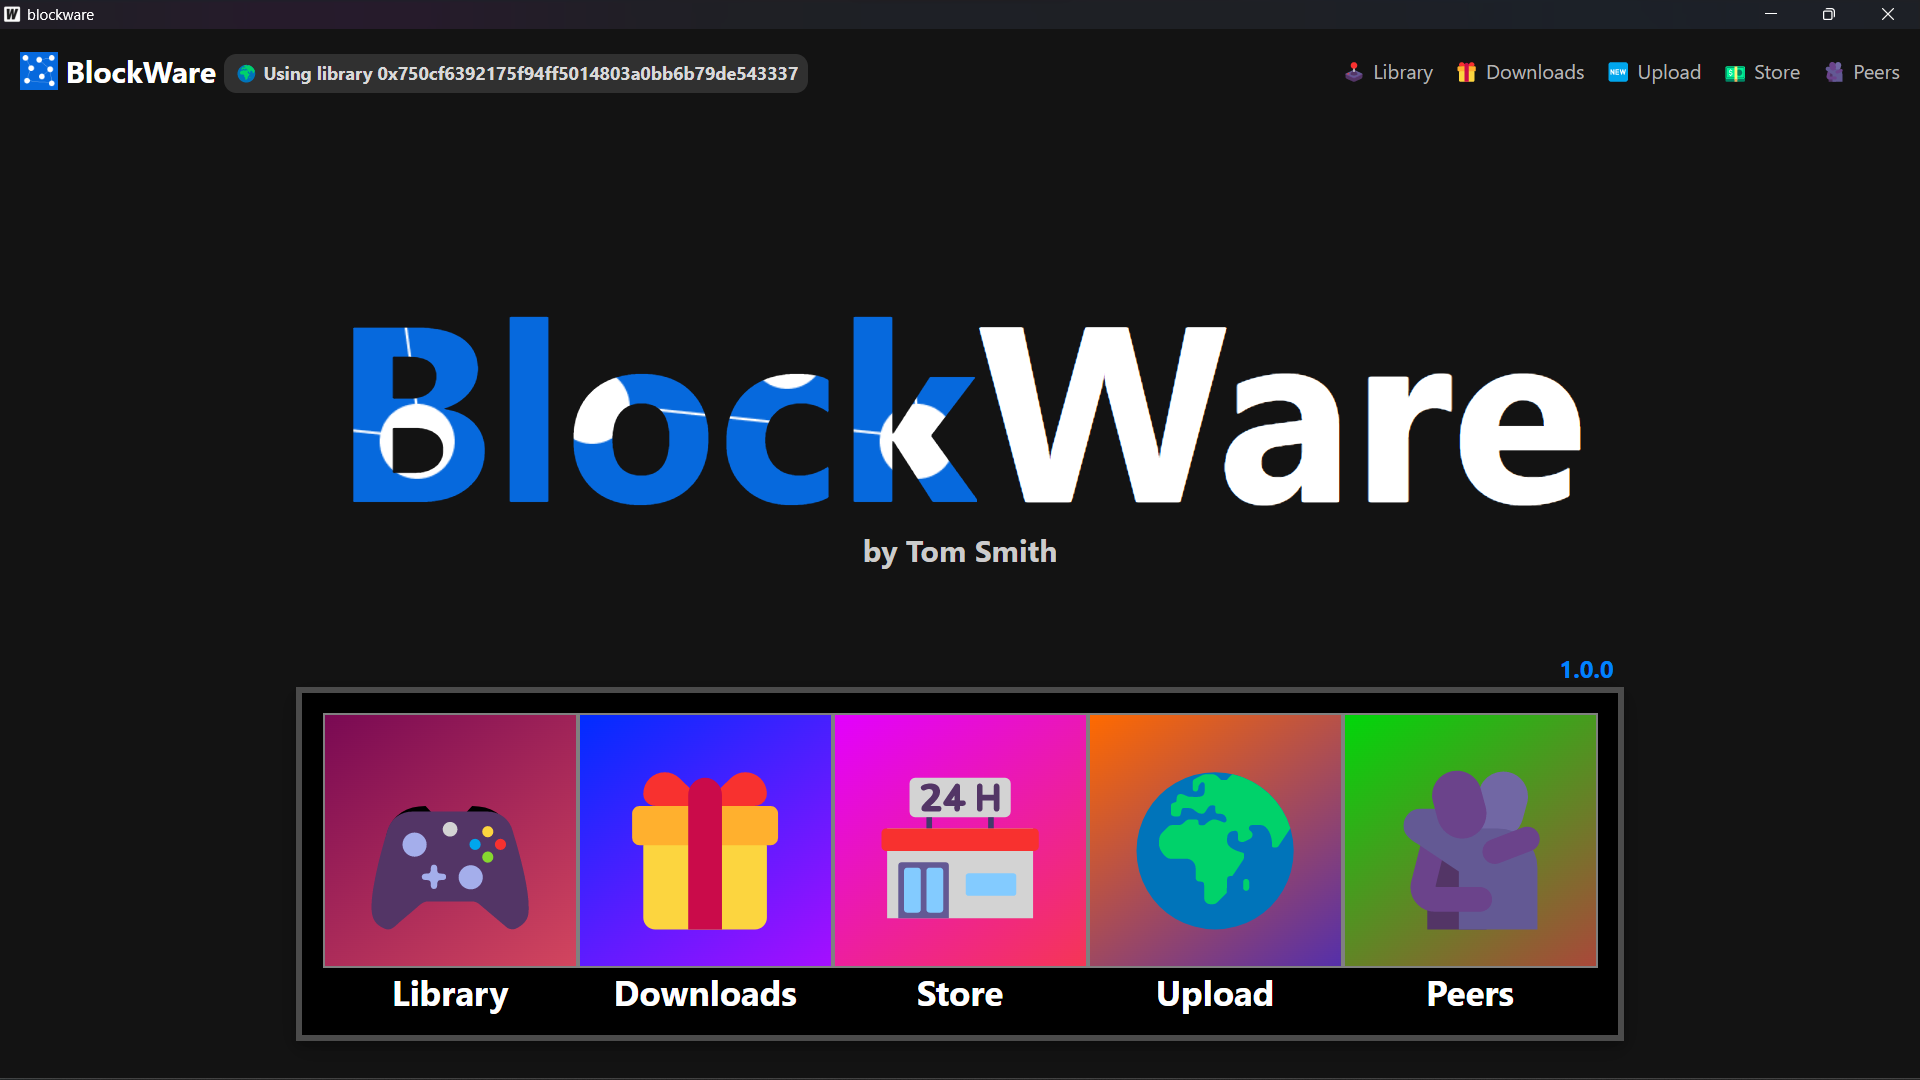
\includegraphics[width=0.9\textwidth]{assets/images/screenshots/home.png}
  \caption{The home page where users can navigate between the main pages.}
\end{figure}

\begin{figure}[H]
  \centering
  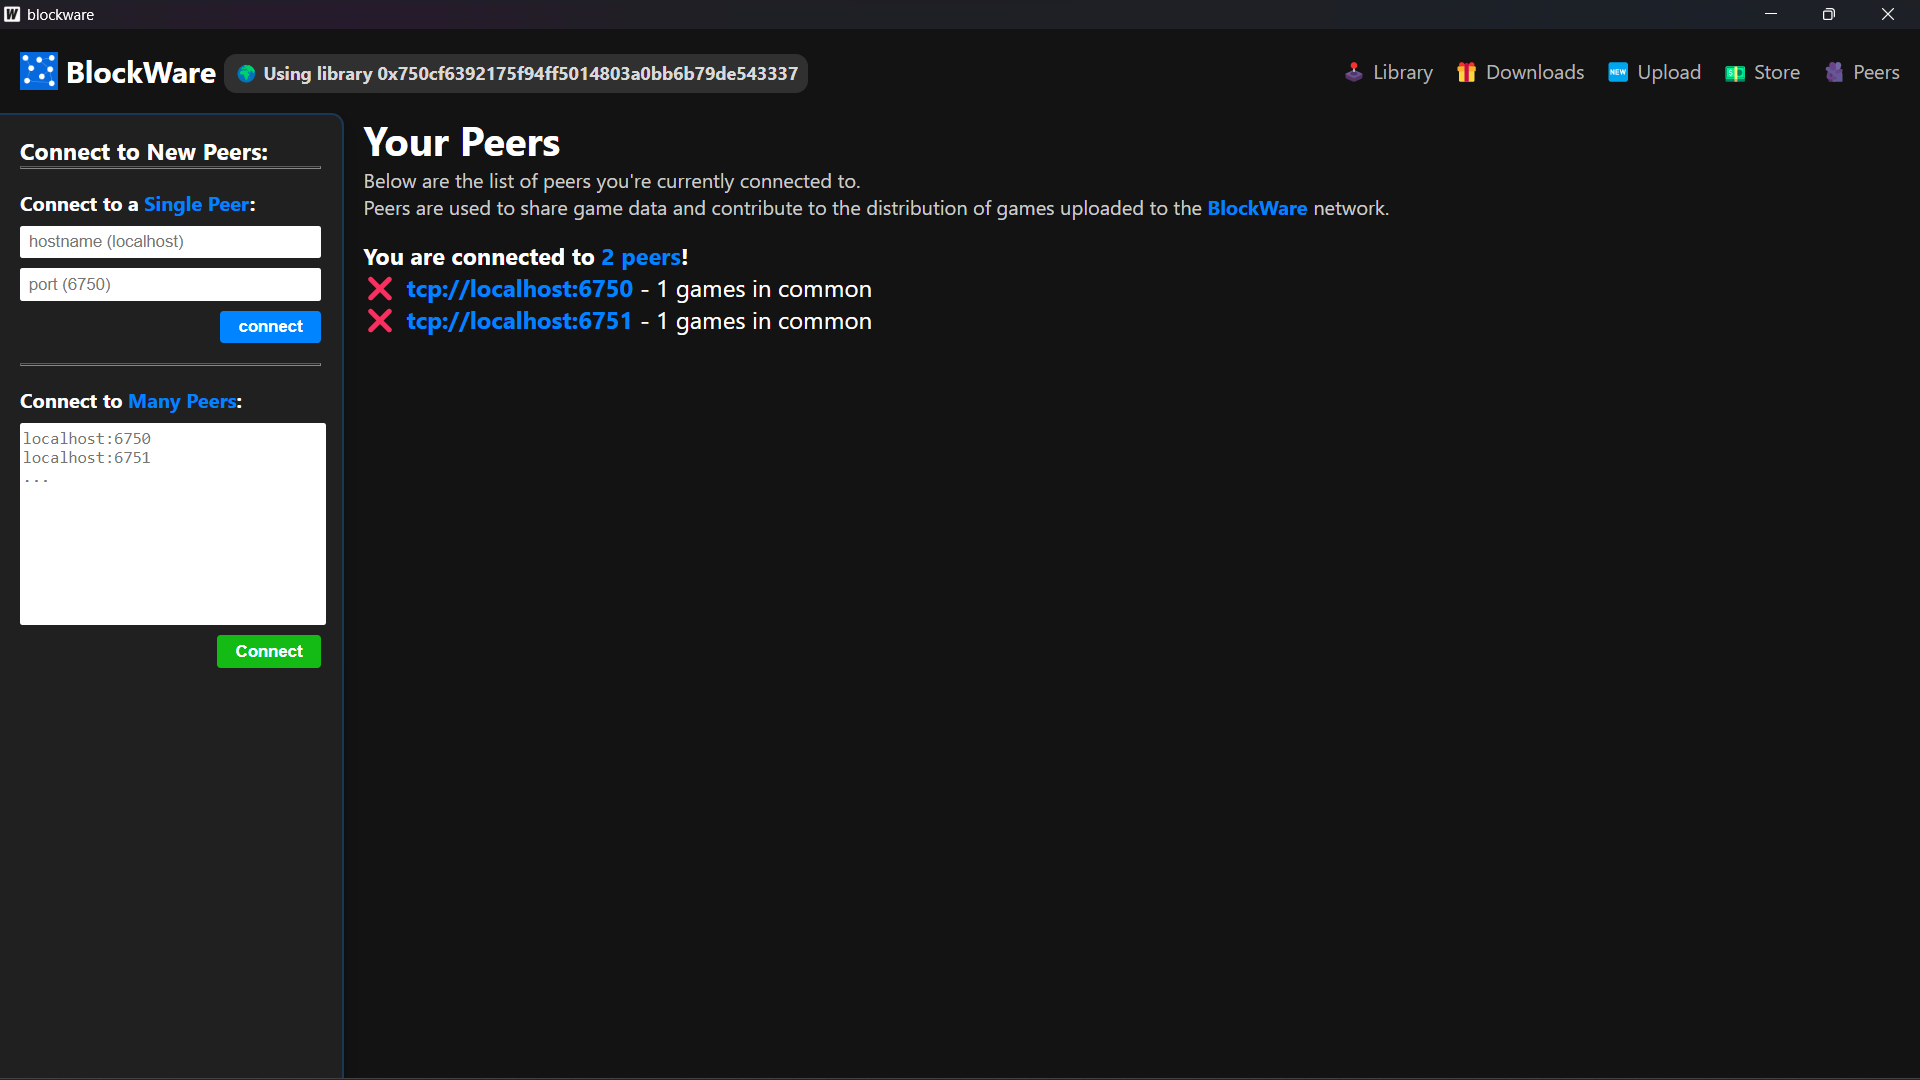
\includegraphics[width=0.9\textwidth]{assets/images/screenshots/peers.png}
  \caption{The page where users can manage their connections to peers with whom they will download game data off of. Users can request receipts from peers that show the amount of data they've sent.}
\end{figure}

\begin{figure}[H]
  \centering
  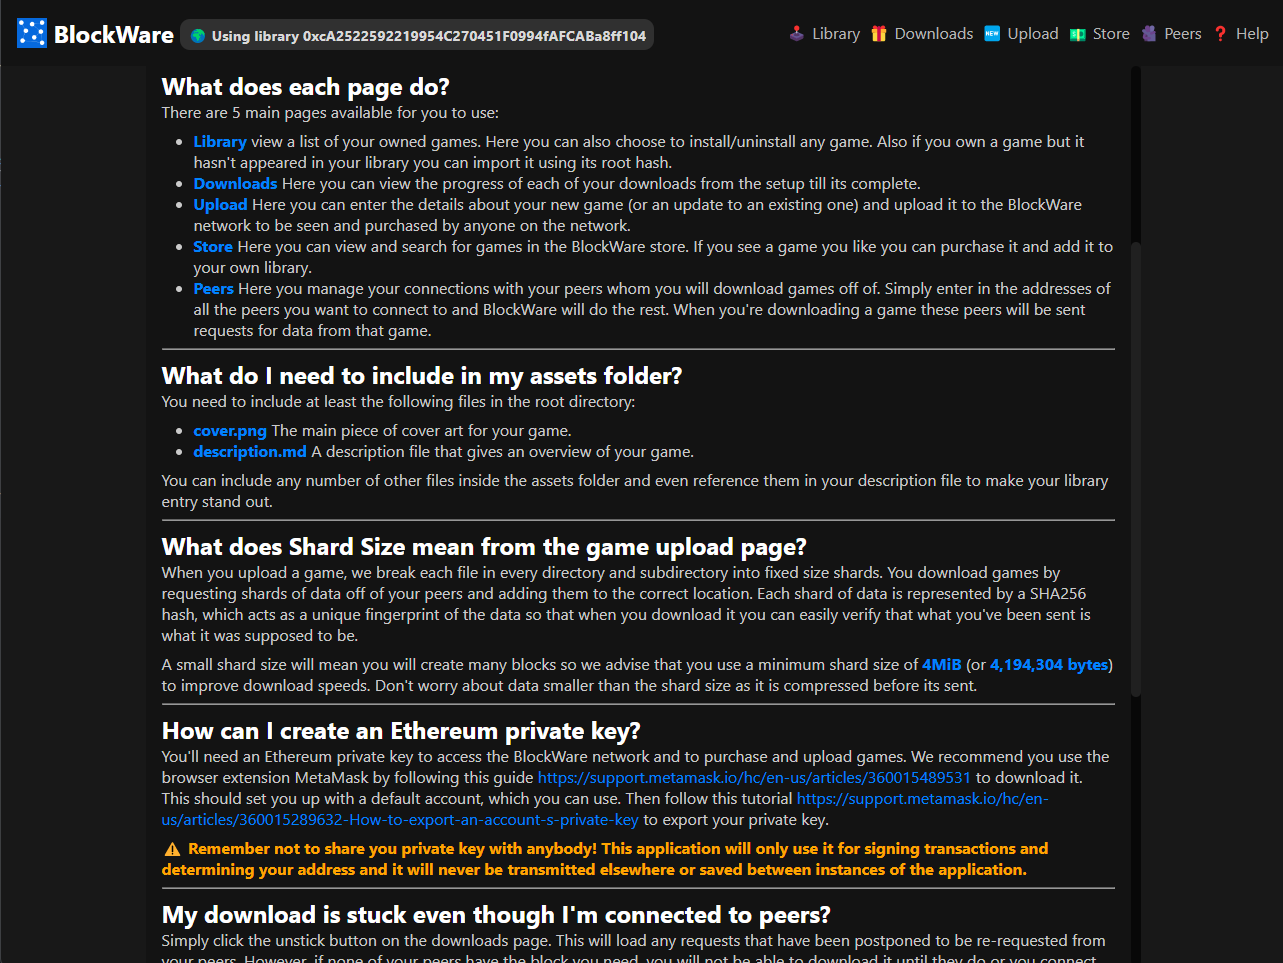
\includegraphics[width=0.9\textwidth]{assets/images/screenshots/help.png}
  \caption{This page has a list of common questions, about the application, expected by users with answers.}
\end{figure}

\begin{figure}[H]
  \centering
  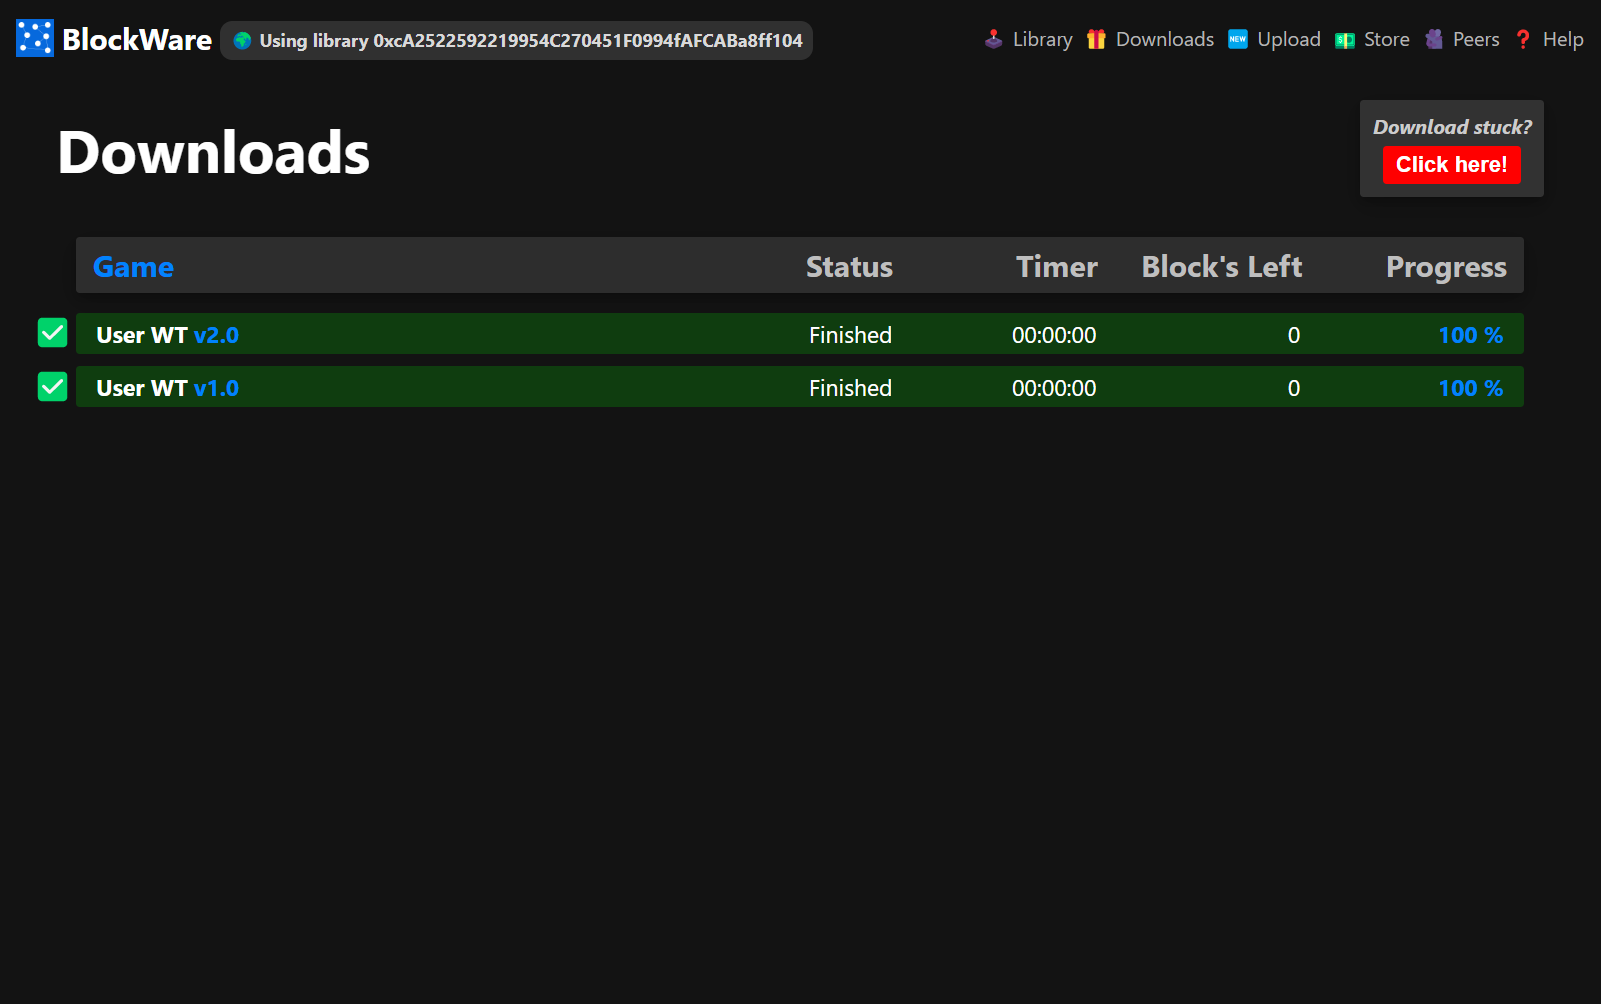
\includegraphics[width=0.9\textwidth]{assets/images/screenshots/downloads.png}
  \caption{This page is where users can track their downloads. It will update in real-time as data is downloaded.}
\end{figure}

\begin{figure}[H]
  \centering
  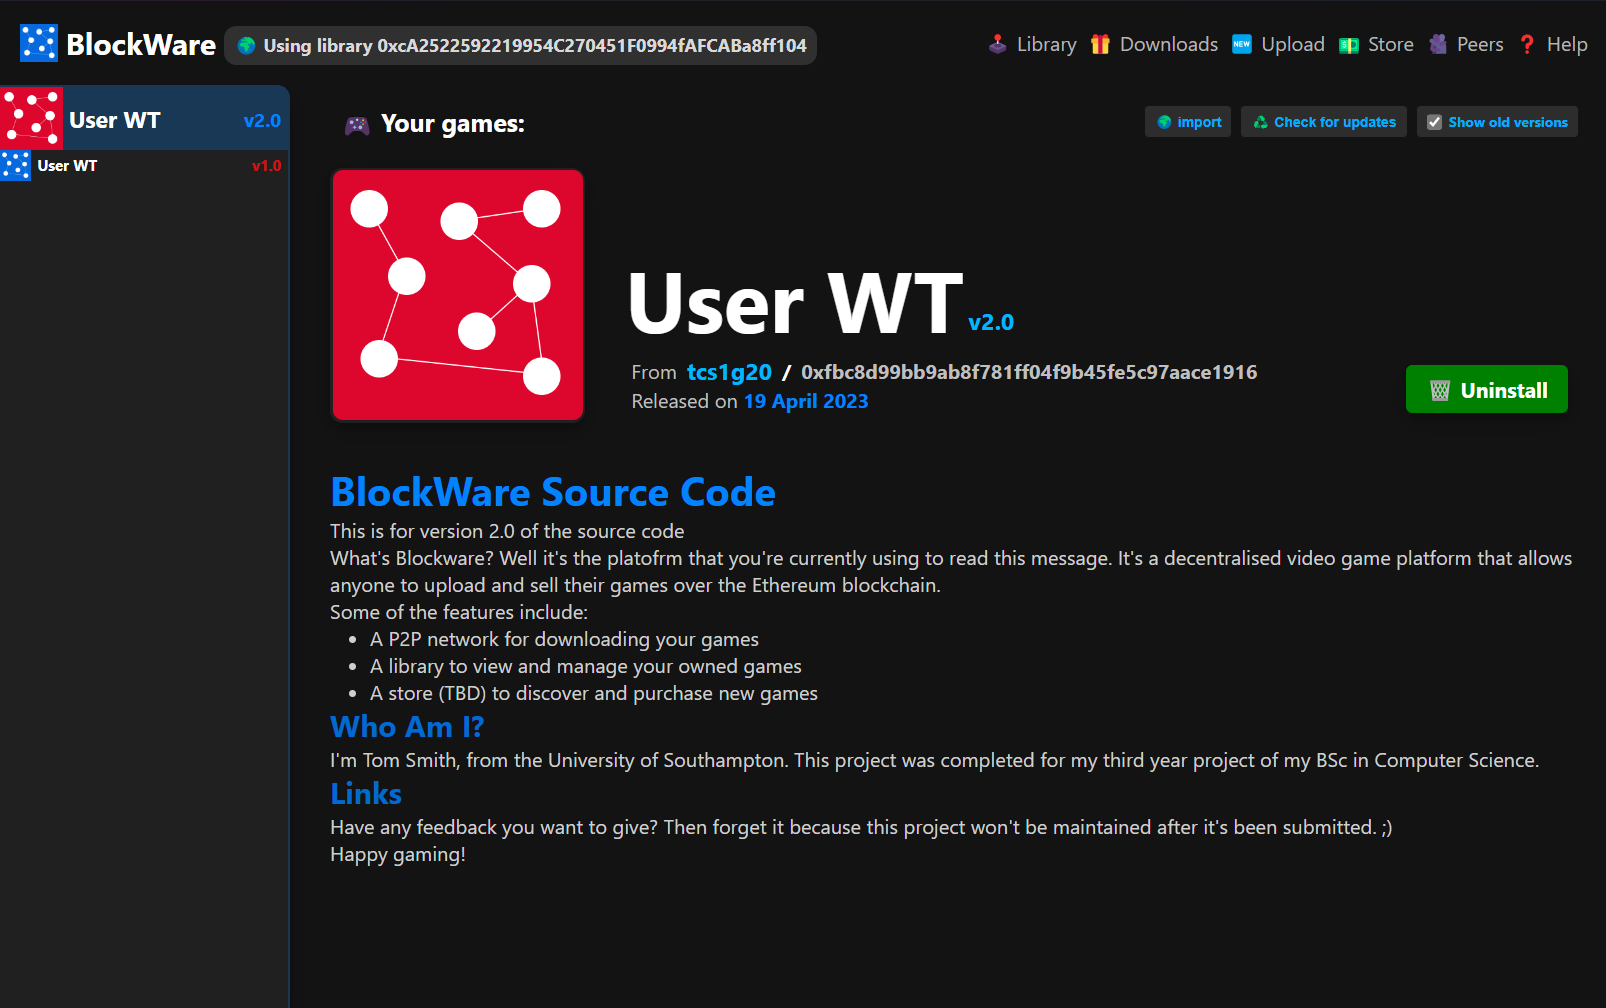
\includegraphics[width=0.9\textwidth]{assets/images/screenshots/library.png}
  \caption{This page shows the user's library of games and allows them to view the assets for them. Smaller games represent older versions of the game and these can be hidden using a the `show old versions' toggle.}
\end{figure}







\chapter{Other Figures}

\section*{Requirement Analysis}\label{app:req-analysis}

Figure~\ref{fig:req-generator} shows a mind-map which shows the relationships between primary stakeholders, key pieces of data and key technologies that were expected to be of use for this project. This allowed me to come up with a suitable set of requirements.

\begin{figure}[ht]
  \centering
  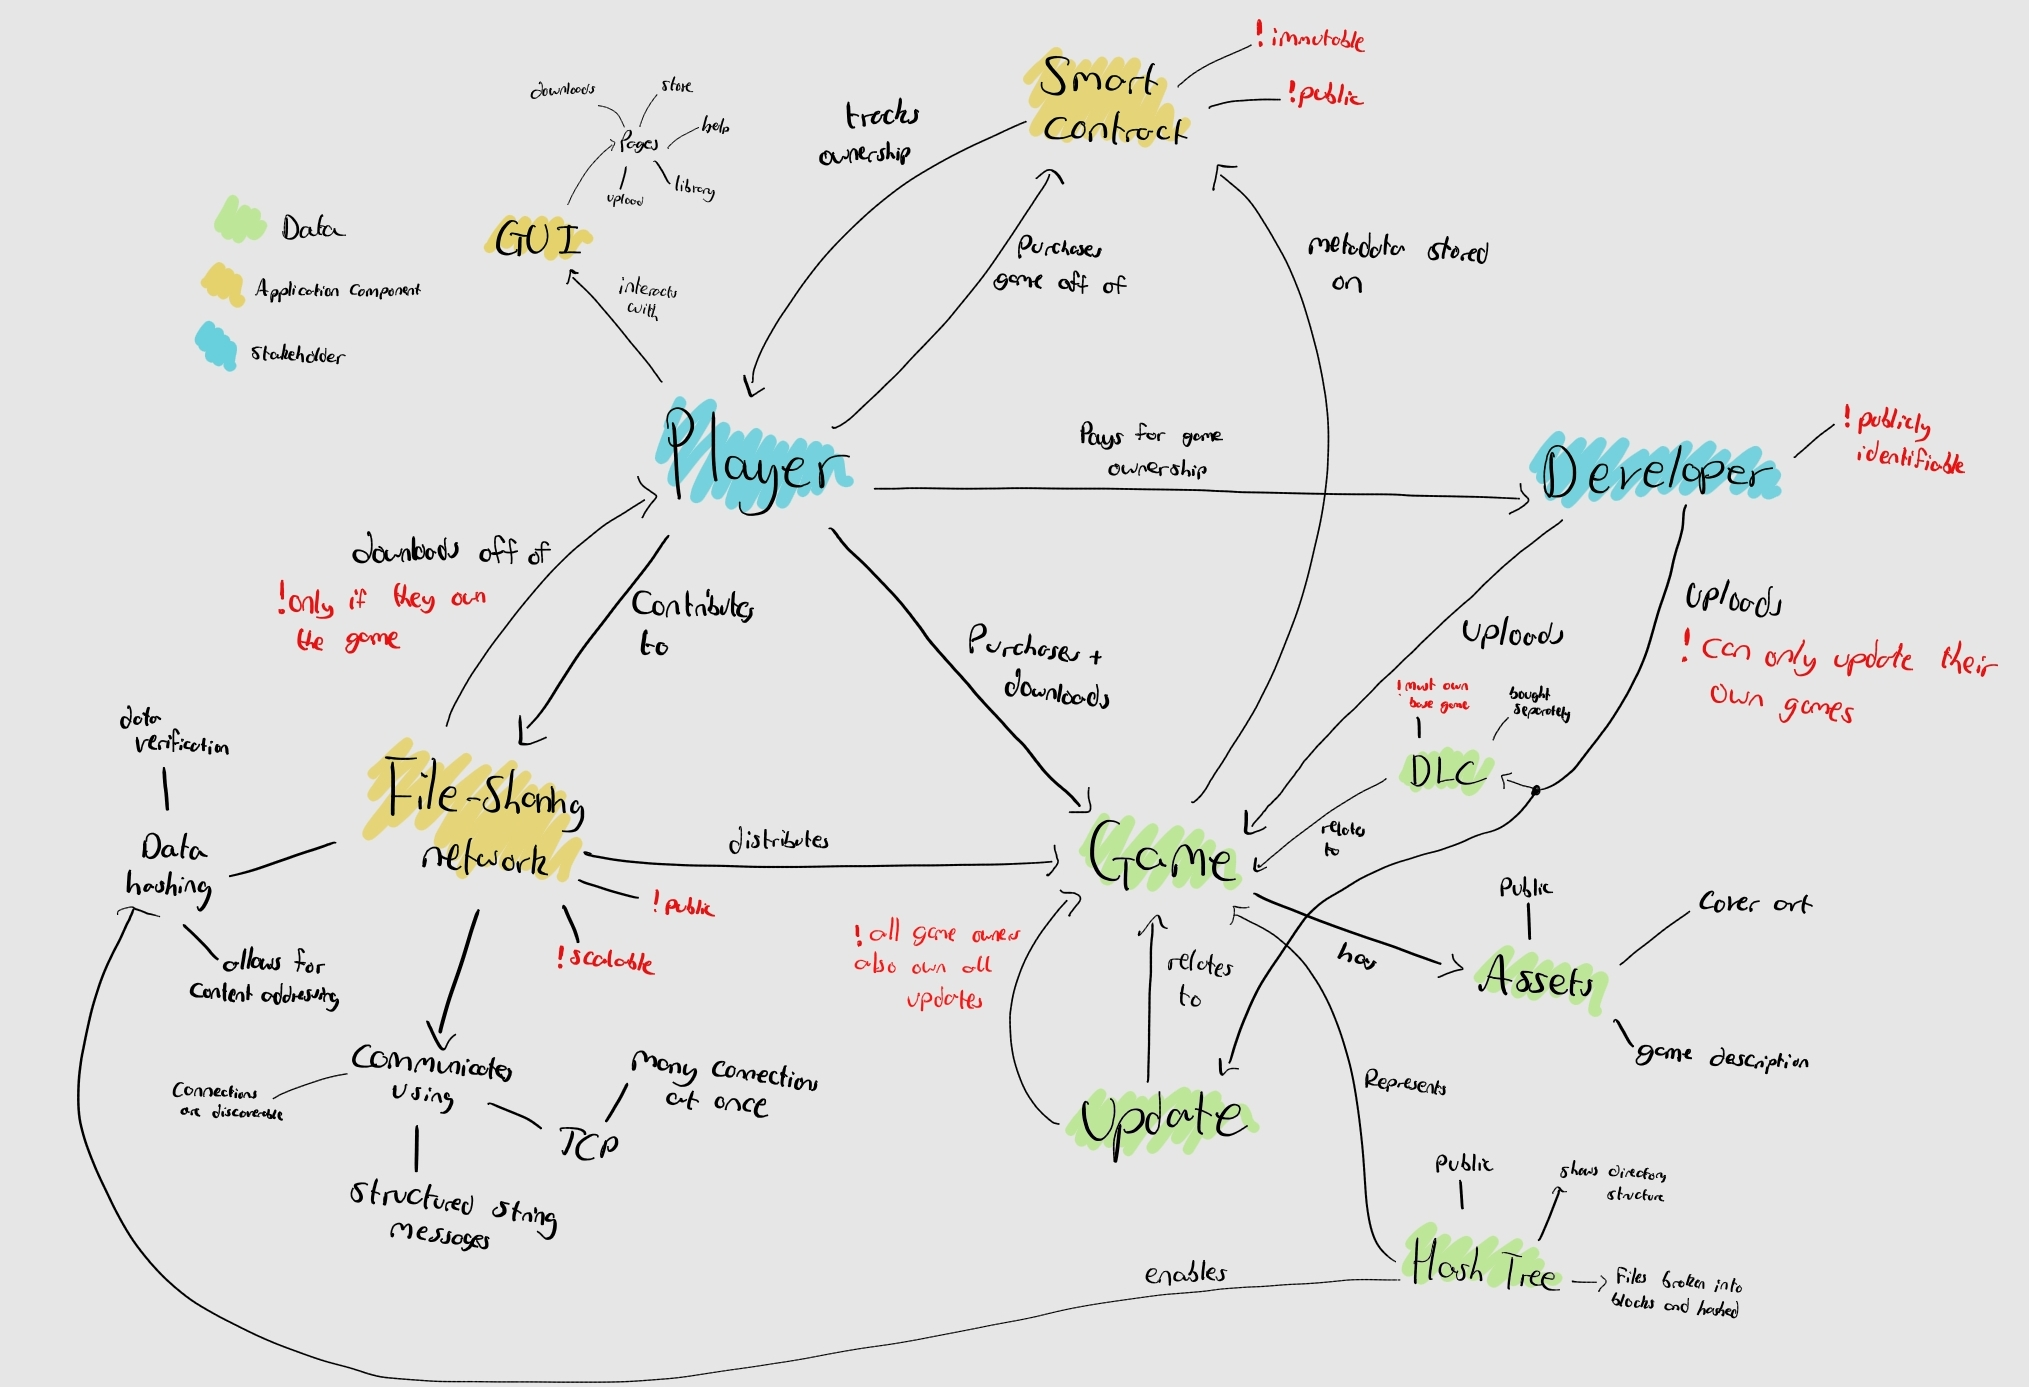
\includegraphics[width=.9\textwidth]{assets/images/diagrams/requirement-generation.jpg}
  \caption{How key elements of the project are related to each other. This diagram was used to help determine the requirements for the application.}
  \label{fig:req-generator}
\end{figure}

\section*{Lines of Code}

Table~\ref{tab:cloc} shows a breakdown of my project by lines of code calculated using CLOC \url{https://github.com/AlDanial/cloc}. 

\begin{longtable}{ r r r r }
  \toprule
  \textbf{Language} & \textbf{Files} & \textbf{Comments} & \textbf{Code}
  \\\midrule\midrule
  Go
  & 44
  & 683
  & 4621
  \\
  Go Tests
  & 29
  & 791
  & 3205
  \\
  Vue.js Components
  & 18
  & 147
  & 2855
  \\
  JavaScript
  & 19
  & 74
  & 209
  \\
  Solidity
  & 1
  & 30
  & 51
  \\\bottomrule\bottomrule
  \caption{The lines of code written for this project calculated excluding any auto-generated code.}
  \label{tab:cloc}
\end{longtable}


\chapter{Progress Report}\label{app:interim}

The rest of this report will show the body of submitted interim report.

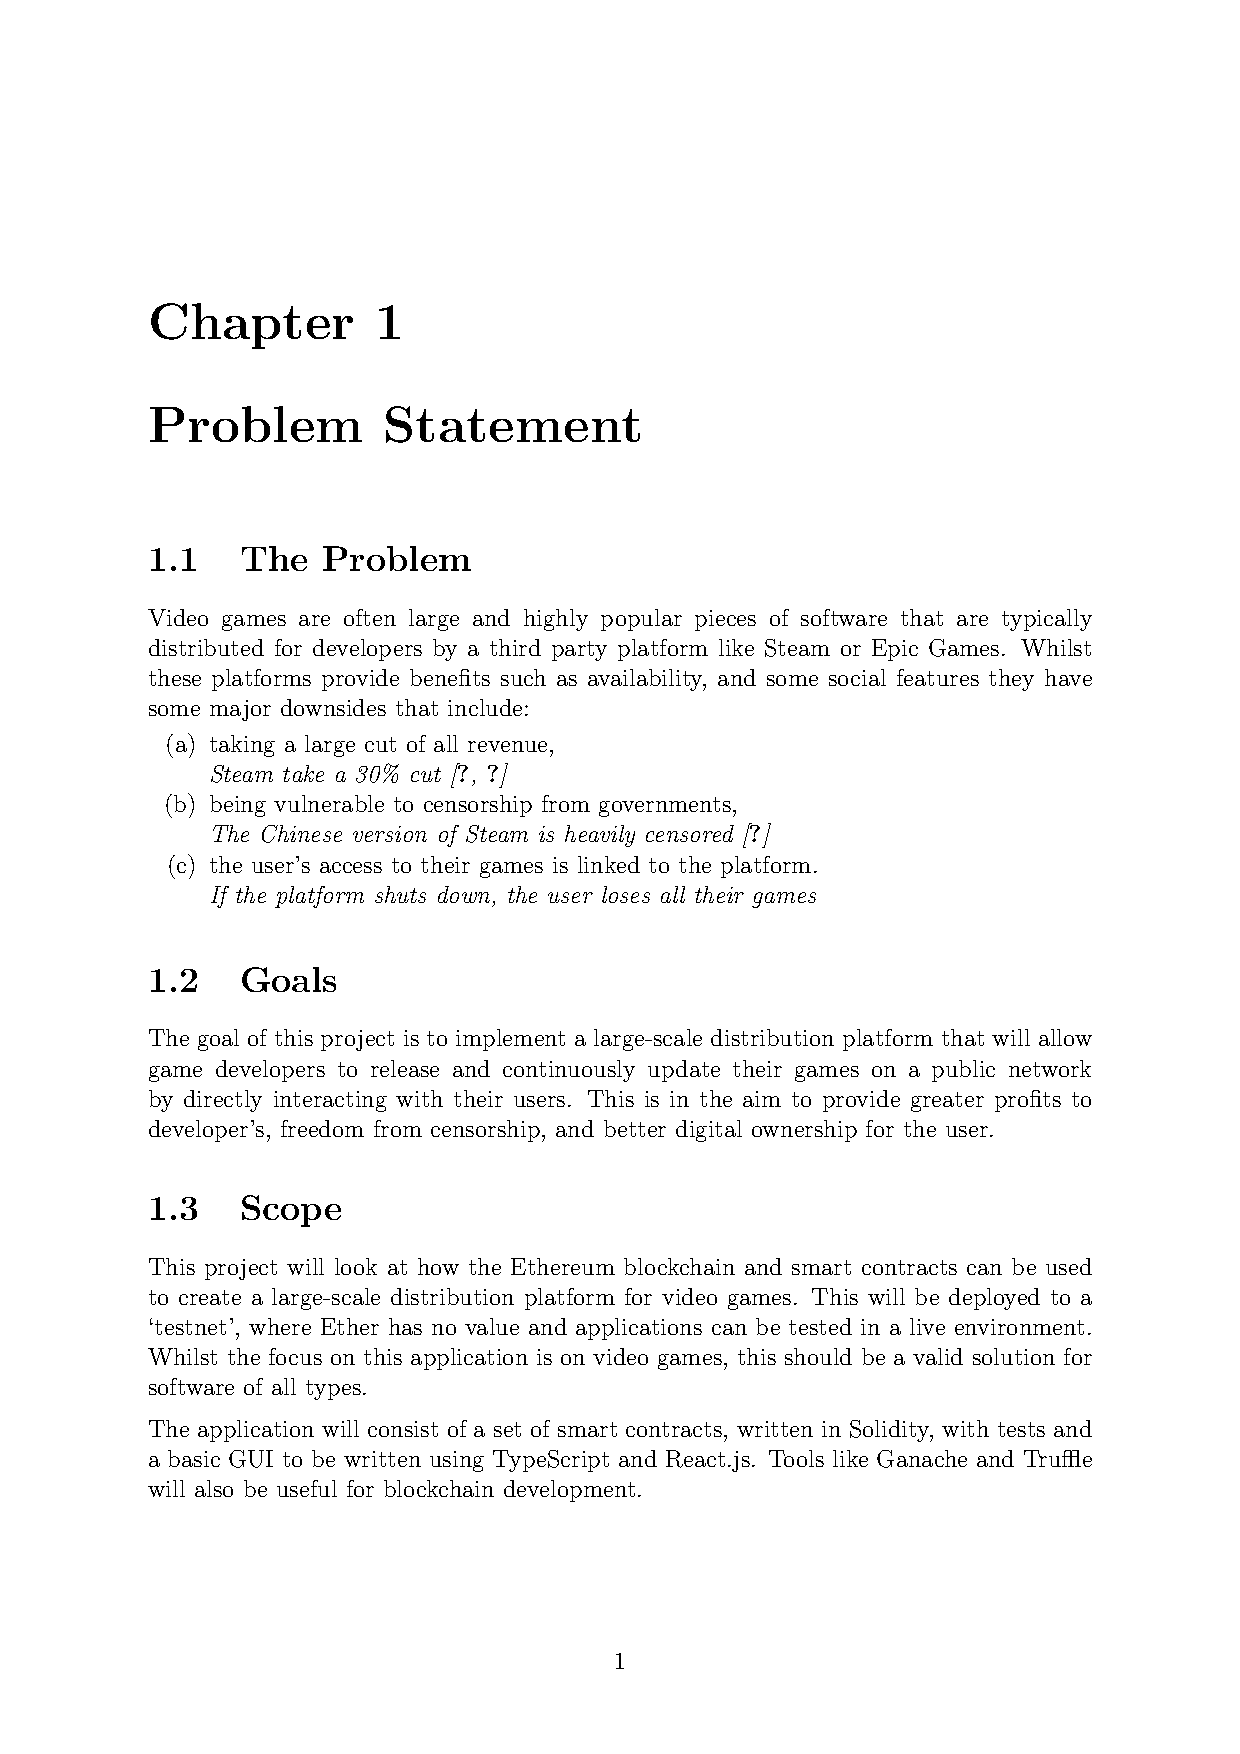
\includepdf[pages=-]{assets/InterimBody.pdf}